%%% DOCUMENTCLASS
\documentclass[letterpaper,twoside,12pt]{report}
\renewcommand{\rmdefault}{bch}

%%% PACKAGES
\usepackage{mdwlist}
\usepackage{amsmath, amsthm, amssymb}
\usepackage{fancyhdr}
\usepackage{graphicx}
\usepackage{listings}
\usepackage{setspace}
%\usepackage[normalsize]{subfigure} %[normalsize]
\usepackage{booktabs}
\usepackage{mathtools}
\usepackage{times}
\usepackage{multicol}
\usepackage{multirow}

\usepackage{caption}
\usepackage[labelformat=simple]{subcaption}
\renewcommand\thesubfigure{(\alph{subfigure})}
%\captionsetup{subrefformat=parens}

\PassOptionsToPackage{hyphens}{url}\usepackage[colorlinks=true, linkcolor=black, citecolor=black, pdftitle={On-Chip Diagnosis of Generalized Delay Failures using Compact Fault Dictionaries}, pdfauthor={Matthew Layne Beckler}, pdfsubject={}, pdfkeywords={}]{hyperref}
\usepackage{breakurl}

\usepackage{xspace}

\usepackage{algorithm}
\usepackage{algorithmic}
\renewcommand{\algorithmiccomment}[1]{// #1}

\hyphenation{micro-archi-tecture}

% another code listing package
% http://stackoverflow.com/a/742012
\lstset{
language=C,
basicstyle=\small\sffamily,
numbers=left,
numberstyle=\tiny,
frame=tb,
columns=fullflexible,
showstringspaces=false
}

\newcommand{\sectionline}{
    \nointerlineskip \vspace{\baselineskip}
    \hspace{\fill}\rule{0.5\linewidth}{.7pt}\hspace{\fill}
    \par\nointerlineskip \vspace{\baselineskip}
}

\graphicspath{{figures/}}
\DeclareGraphicsExtensions{.pdf,.jpg,.jpeg,.png}


% %%% SPACING
\doublespacing
%\onehalfspacing

% %%% PAGE FORMAT
\oddsidemargin 0.2in
\evensidemargin 0.2in
\topmargin 0.0in
\headheight 15pt
%\headheight 0.0in
\textwidth  6in
\textheight 9in
\hoffset 0.0in
%\voffset -.55in
\voffset -.5in
\footskip .25in

% \hoffset .25in


% %%% HEADERS & FOOTERS
\pagestyle{fancy} % options: empty, plain, fancy
\pagenumbering{arabic}
\renewcommand{\headrulewidth}{0.4pt}
\fancyhead[RE,LO]{\bf \thepage}
\fancyhead[RO]{\bf \leftmark}
\fancyhead[LE]{\bf \rightmark}
\fancyfoot[C]{}

\renewcommand{\sectionmark}[1]{ \markright{\thesection.\ \ #1}}
\renewcommand{\chaptermark}[1]{ \markboth{\chaptername\ \thechapter.\ \ #1}{}}

% allow align to break if it needs to
%\allowdisplaybreaks[1]


\begin{document}
%\input{utils}

%%% TITLEPAGE
\begin{titlepage}
\begin{center}

\singlespacing

%%\centering
\vspace*{1.0in}

{\large \bf On-Chip Diagnosis of Generalized Delay Failures\\using Compact Fault Dictionaries}

\vspace{1in}

{\doublespacing
Submitted in partial fulfillment of the requirements for \\
the degree of \\
Doctor of Philosophy \\
in \\
Electrical and Computer Engineering }

\vspace{1.3in}

Matthew Layne Beckler
\\[\baselineskip]
B.S., Computer Engineering, University of Minnesota\\
M.S., Electrical and Computer Engineering, Carnegie Mellon University

\vspace{1.8in}

Carnegie Mellon University \\
Pittsburgh, PA
\\[\baselineskip]
April, 2017

\vfill
\end{center}
\end{titlepage}
\raggedbottom

\pagenumbering{roman}


\pagenumbering{roman}

%%% COPYRIGHT PAGE
\begin{titlepage}
\begin{center}
\vspace*{\fill}
Copyright \copyright~2017

Matthew Layne Beckler

All rights reserved
\vspace*{\fill}
\end{center}
\end{titlepage}

%%% ABSTRACT
\pagenumbering{roman}

\chapter*{Acknowledgments}
My sincerest thanks to my academic advisor, Professor Shawn Blanton.
%
I am deeply grateful for his continued support and patience as I struggled through this long process.
%
He has given me valuable instruction not only in the technical aspects of this particular domain, but wider lessons on academic research and writing, while providing constant encouragement and a positive attitude.
%
This thesis would not have been possible without his guidance and advice.

I would like to thank the other members of my committee, Prof. Ken Mai, Prof. Diana Marculescu, and Prof. Subhasish Mitra, for finding time to share their knowledge and advice as part of my thesis committee.
%
Their suggestions, ideas, and feedback have helped me to focus the ideas we originally discussed during my thesis proposal into this final product.

Many thanks to the dedicated staff of the ECE department, including Adam Palko, Judy Bandola, Elaine Lawrence, Susan Farrington, Samantha Goldstein, and Nathan Snizaski.
%


I am sincerely grateful to all past and present ACTL students, including Jeff Nelson, Osei Poku, Yen-Tzu Lin, Wing-Chiu Tam, Xiaochun Yu, John Porche, Mitch Martin, Hongfei Wang, Cheng Xue, Xuanle Ren, Ben Niewenhuis, and Martyn Romanko - Your friendship and assistance during our years together was invaluable.
%
Special thanks to Ben Niewenhuis and Harsh Shrivastava for their research contributions.
%
Also thanks to other ECE grad students including Peter Klemperer, Adam Hartman, Kristen Dorsey, John Kelly, Craig Teegarden, Scott Fisk, Stephen Powell, Joey Fernandez, Mark McCartney, Peter Milder, and everyone else I am forgetting here - I sincerely enjoyed the many shared meals, cups of coffee, and camaraderie.
%
Many thanks to the ECE Graduate Organization for organizing social events and providing opportunities for volunteer service.
%
Further thanks to the ECE department softball team (The Gigahurtz), for getting the pale nerds outside in the fresh air once in a while.
%
Thanks to Dr. Yanjing Li for our many fruitful discussions of on-chip test, NBTI, ELF, and many other topics through the years.

To my parents Rick and Linda Beckler, who have always supported my wildest dreams and craziest plans, thank you for the never-ending support.
%
Thank you for all the encouragement through this whole process, your visits to Pittsburgh, and the excellent holidays away from school.

Finally, this dissertation is dedicated to my dearest wife, Anna.
%
Thank you for following me across the country and making a life together far from home.
%
Thank you for keeping me sane during this journey, and sticking it out with me until the end.
%
Thank you for your endless love and support, I could not have done this without you.

\sectionline

The work in this dissertation was supported by the Semiconductor Research Corporation through contract no. 1974.001, the National Science Foundation under contract no. 0903478, as well as the Lamme/Westinghouse and Bertucci Graduate Fellowships.



\newpage

\section*{Abstract}
Integrated Circuits (ICs) are an essential part of nearly every electronic device.
%
From toys to appliances, spacecraft to power plants, modern society truly depends on the reliable operation of billions of ICs around the world.
%
The steady shrinking of IC transistors over past decades has enabled drastic improvements in IC performance while reducing area and power consumption.
%
However, with continued scaling of semiconductor fabrication processes, failure sources of many types are becoming more pronounced and are increasingly affecting system operation.
%
Additionally, increasing variation during fabrication also increases the difficulty of yielding chips in a cost-effective manner.
%
Finally, phenomena such as early-life and wear-out failures pose new challenges to ensuring robustness.

One approach for ensuring robustness centers on performing test during run-time, identifying the location of any defects, and repairing, replacing, or avoiding the affected portion of the system.
%
Leveraging the existing design-for-testability (DFT) structures, thorough tests that target these delay defects are applied using the scan logic.
%
Testing is performed periodically to minimize user-perceived performance loss, and if testing detects any failures, on-chip diagnosis is performed to localize the defect to the level of repair, replacement, or avoidance.

In this dissertation, an on-chip diagnosis solution using a fault dictionary is described and validated through a large variety of experiments.
%
Conventional fault dictionary approaches can be used to locate failures but are limited to simplistic fail behaviors due to the significant computational resources required for dictionary generation and memory storage.
%
To capture the misbehaviors expected from scaled technologies, including early-life and wear-out failures, the Transition-X (TRAX) fault model is introduced.
%
Similar to a transition fault, a TRAX fault is activated by a signal level transition or glitch, and produces the unknown value \textit{X} when activated.
%
Recognizing that the limited options for runtime recovery of defective hardware relax the conventional requirements for defect localization, a new fault dictionary is developed to provide diagnosis localization only to the required level of the design hierarchy.
%
On-chip diagnosis using such a hierarchical dictionary is performed using a new scalable hardware architecture.
%
To reduce the computation time required to generate the TRAX hierarchical dictionary for large designs, the incredible parallelism of graphics processing units (GPUs) is harnessed to provide an efficient fault simulation engine for dictionary construction.
%
Finally, the on-chip diagnosis process is evaluated for suitability in providing accurate diagnosis results even when multiple concurrent defects are affecting a circuit.


\newpage

\tableofcontents
\listoftables
\listoffigures
\listofalgorithms
\clearpage

% If need a blank page get Page 1 to be left-handed.  Get rid of line and header,
% make an empty page, go to next page, turn headers back on, continue.
\renewcommand{\headrulewidth}{0pt}
\fancyhf{}
\mbox{}
\newpage
\pagestyle{fancy}
\pagenumbering{arabic}
\renewcommand{\headrulewidth}{0.4pt}
\fancyhead[RE,LO]{\bf \thepage}
\fancyhead[RO]{\bf \leftmark}
\fancyhead[LE]{\bf \rightmark}
\fancyfoot[C]{}



\pagenumbering{arabic}
\setcounter{page}{1}

\chapter{Introduction}
\label{chap:intro}

Integrated Circuits (ICs) are an essential part of nearly every electronic device.
%
From toys to appliances, spacecraft to power plants, modern society truly depends on the reliable operation of billions of ICs around the world.
%
The steady shrinking of IC transistors over past decades has enabled drastic improvements in IC performance while reducing area and power consumption.

However, this continual scaling-down has not been free from downsides.
%
IC manufacturing is a very complex process involving hundreds of discrete steps, with additional steps and complexity added with each feature size shrink.
%
A variety of failure sources are now becoming more pronounced~\cite{srinivasan04}, and are having a larger effect on correct system operation~\cite{itrspids,karnik02}.
%
Increasing variation in the manufacturing process~\cite{borkar03} also means that yielding chips cost-effectively becomes even more challenging.
%
In addition, phenomena such as early-life and wear-out failures pose new challenges to ensuring robustness~\cite{borkar03,itrspids}, where \textit{robustness} is the ability of a system to continue acceptable operation in the presence of various types of misbehaviors over its intended lifetime.

Given the variety of computing systems deployed today, the consequences of a failing system vary widely.
%
While defective consumer electronics can be easily replaced (albeit at some cost to either the manufacturer or customer), other systems can be much more difficult to service.
%
The increasing emergence of life- and safety-critical systems such as autonomous vehicles~\cite{spectrumselfdriving} and long-term implantable electronic medical devices are two examples of performance-driven systems where correct operation is critical, and timely replacement is difficult or impossible.
%
In these situations, robust system design is the best approach to overcome such reliability challenges.

Robust system design is a problem that has been substantially addressed in the past.
%
For example, one conventional method for achieving system robustness is to use a conservative design technique that incorporates speed guardbands.
%
Conservative design, however, results in significant performance loss and is increasingly expensive due to the extreme measures needed to overcome the level of variation exhibited by modern ICs~\cite{jeong09}.
%
At the other extreme, one can aggressively design the IC assuming optimal fabrication conditions, and then use manufacturing test to select ICs that satisfy the specification.
%
Such an approach would lead however to unacceptable cost since yield would likely be extremely low.
%
Traditional fault tolerance could also be employed.
%
However, techniques such as TMR (triple modular redundancy)~\cite{stroud94,radu00} and duplicate-with-compare~\cite{johnson08} are much too expensive in terms of chip overhead and power consumption, especially for the many portable, consumer-oriented systems that are now pervasive.
%
Another class of fault tolerance includes ``always-on'' error-correction techniques.
%
Although there is less area overhead, the level of error-correction needed would consume an excessive amount of power~\cite{siewiorek98}.%TODO more background? Something on software diagnosis?

Another approach being actively investigated~\cite{li08,inoue08,li10casp,li13}, and adopted here for our on-chip architecture, involves periodically testing the system using tests that target the specific behaviors exhibited by known failure sources such as early-life and wear-out failures.
%
In various experiments involving actual test chips~\cite{agarwal07,chen09}, it is demonstrated that both early-life and wear-out failures manifest as delay increases in standard cells.
%
Leveraging the already-existing design-for-testability (DFT) structures, thorough tests that target these delay shifts are brought into the chip and applied structurally (at configurable speeds) using the scan logic.
%
In addition to detecting failure, adjusting the speed of the test also allows impending chip failures to be predicted before they occur.
%
Accelerated testing is an important aspect of this approach because detecting a pending failure using accelerated tests enables us to perform repair, replacement, or avoidance (in general, \textit{recovery}) of the nearly-faulty module before it actually fails.
%
This means the pending failure does not have a chance to affect correct system operation, and a time-consuming roll-back of execution state is not needed.
%
Testing is performed periodically to minimize the user-perceived performance loss while ensuring that the pending failure is detected before it corrupts any system data.
%
If testing detects a failure or pending failure, diagnosis is performed to pinpoint the location of the affected portion of the system.

One method for identifying the failure location, a fault dictionary, can be effective but has a number of drawbacks~\cite{pomeranz97} that include (i) the computation needed to generate the dictionary, (ii) the resulting size of the dictionary that can be easily multiple terabytes for modern designs, and (iii) the conventional use of the single-stuck line fault model~\cite{abramovici90} which significantly degrades diagnostic accuracy due to its mismatch with actual misbehavior.
%
Once a fault dictionary has been constructed, its use for on-chip diagnosis remains a challenge.
%
The on-chip diagnosis architecture should have only a negligible effect on chip performance.
%
For example, if hardware modules must be taken ``off-line'' for test and diagnosis, the duration should be minimized to reduce the performance loss~\cite{li08}.
%
Furthermore, the hardware resources allocated for on-chip diagnosis should be limited and amortized to reduce the area and power impact on the overall chip.

\begin{figure}[hbtp]
\centering
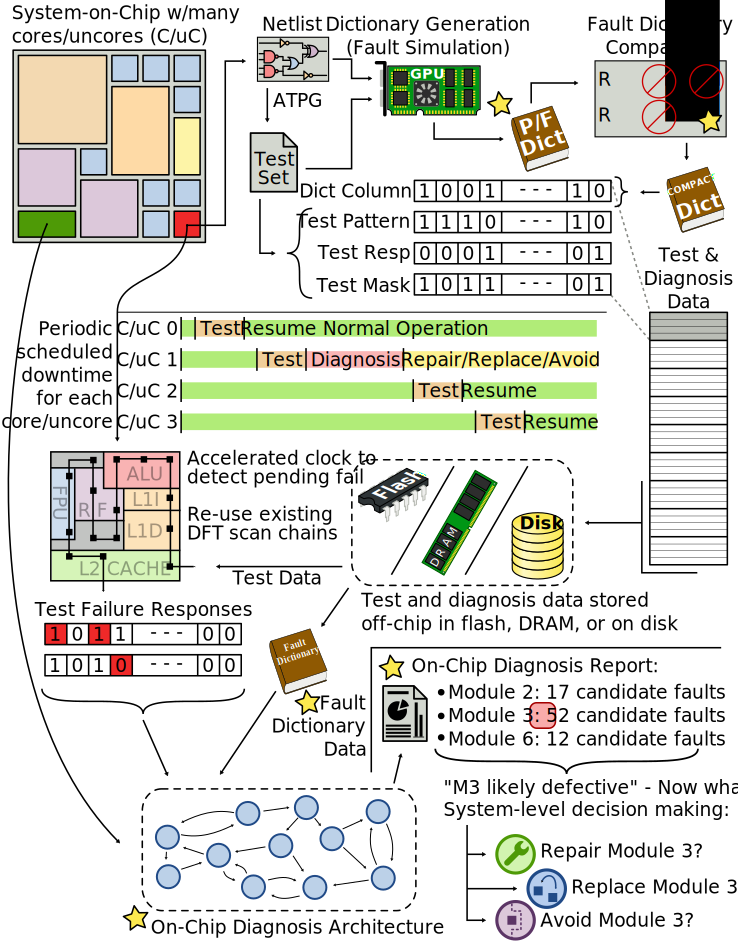
\includegraphics[width=1.0\columnwidth]{fig_intro_supergraphic}
\caption{Overall system test and diagnosis process includes several dissertation contributions (indicated by a yellow star).}
\label{fig:intro_supergraphic}
\end{figure}

Figure~\ref{fig:intro_supergraphic} shows a high-level view of these concepts.
%
While this dissertation does not accomplish everything shown (a yellow star icon indicates dissertation contributions), it is important to understand the overall process into which this dissertation fits.
%
The netlist of each System-on-Chip (SoC) core/uncore is used with Automatic Test Pattern Generation (ATPG) to generate a test set.
%
GPU-accelerated fault simulation analyzes the core/uncore netlist and test set to produce the pass/fail dictionary, further processed by dictionary compaction to produce the compacted pass/fail dictionary.
%
This pre-computed test and diagnosis data (consisting of the test pattern, test response, test mask, and fault dictionary data) is stored off-chip in flash, DRAM, or on disk.
%
The on-chip test controller~\cite{li13} schedules periodic testing downtime, for each core/uncore in the system.
%
The corresponding test data is applied to the core/uncore under test, re-using existing DFT structures such as scan chains and/or boundary scan.
%
The on-chip diagnosis architecture uses the hierarchical fault dictionary data to analyze the failing test responses to determine the set of candidate faults, grouped by repair-level module.
%
These per-module candidate fault counts are provided to the system-level for decision making, for example, to choose between repair, replacement, or avoidance of the most likely defective module(s).

\section{System Test and Diagnosis}
\label{sec:intro_system_test_and_diag}

Knowing that a system has failed (or will fail) is not sufficient to ensure robustness.
%
Beyond failure detection, there must also be a way to replace the faulty system component, repair the system, or to continue operation while avoiding the faulty circuitry.
%
One example of system repair is detailed in~\cite{li13}, where non-processor System-on-Chip (SoC) components such as cache and memory controllers (so-called \textit{uncore} components) are enhanced with self-repair capabilities.
%
The two repair techniques described in~\cite{li13} include (i) resource reallocation and sharing, where \textit{helper} components are reconfigured to share the workload of the faulty component, and (ii) sub-component logic sparing, where the design hierarchy is traversed to identify identical sub-components that could share logic spares.
%
Using both of these techniques, the authors of~\cite{li13} achieve self-repair coverage of 97.5\% with only 7.5\% area and 3\% power overhead for the OpenSPARC T2 processor design~\cite{sun11}.

Before a repair technique can be applied, however, the location of the faulty circuit must be identified.
%
Moreover, the identification process must be performed in-situ, since it is unlikely it can be accomplished off-chip without affecting system performance.
%
The process of identifying the failure location is known as \textit{diagnosis}.
%
In diagnosis, the conventional objective is to identify a fault site corresponding to the actual failure location.
%
Two categories of approaches exist for diagnosis.
%
In effect-cause diagnosis, a complete model of the design, its test-vector set, and the test response from the failing circuit are analyzed by diagnostic software to identify possible fault locations.
%
All commercial EDA vendors offer powerful software tools for diagnosing modern designs using effect-cause approaches.
%
An effect-cause approach for on-chip diagnosis is likely infeasible since the amount of memory and run-time for modern designs can be extremely large.
%
For example, merely loading the netlist image of a modern design into memory can take more than an hour.

The other approach to diagnosis is known as cause-effect, where all faults are simulated to create a cataloging or \textit{dictionary} of all possible test responses.
%
Diagnosis compares the actual circuit-failure response with all the fault-simulation responses stored in the dictionary.
%
Fault sites with a response that matches or closely matches the actual failing-circuit response are identified as likely failure locations.
%
Ideally, only one fault site is reported.

Unlike effect-cause approaches, the actual task of using a dictionary does not require a complex software analysis tool.
%
Instead, the significant task of creating the dictionary is performed only once, off-line, before the design is even fabricated, thus allowing the immense computation required to be amortized over all systems that will utilize the dictionary.
%
Performing diagnosis using a dictionary consists of lookups, which in an on-chip environment, can be efficiently accomplished by storing the dictionary in off-chip memory.

Conventional fault dictionaries are not perfect however in that they suffer from three significant drawbacks.
%
First, as mentioned, the generation time is significant.
%
This is because every fault is simulated using all test patterns (i.e., there is no fault dropping), and the complete fault response needs to be generated in the most general case.
%
Second, since the entire response for every possible fault is stored in the dictionary, its size can be huge.
%
Finally, because the dictionary size is a tremendous challenge, the fault model employed must have a limited universe (e.g., on par with the stuck-at model).
%
The consequence of using a simple fault model means however that it is much more likely that the actual circuit-failure response will differ significantly from any of the modeled fault responses stored in the dictionary.

Despite these drawbacks, dictionaries are the best choice for on-chip diagnosis since these disadvantages can be mitigated.
%
Specifically, the cost associated with dictionary generation can be amortized across the lifetimes of all the systems that will use the dictionary for on-chip diagnosis.
%
Dictionary size can be substantially reduced using conventional techniques, and by reducing the number of faults in the dictionary through a new form of collapsing that exploits the granularity of repair.
%
Additionally, advanced computational resources such as Graphics Processing Units (GPUs) can exploit the highly-parallel nature of fault simulation to drastically reduce the amount of time required for dictionary generation.
%
Finally, the failure-fault mismatch problem is handled through the use of an enhanced delay-fault model that conservatively captures the possible misbehaviors exhibited by early-life and wear-out failures without increasing the size beyond the stuck-at fault universe.

It is important to consider the differences between the goals of conventional fault diagnosis and the goals of on-chip diagnosis.
%
In conventional fault diagnosis, the focus is on process improvement or low-level design improvement via physical failure analysis (PFA) of the sites reported by diagnosis.
%
PFA requires a precise result, ideally the actual $(x, y, z)$ location of the failure.
%
The on-chip diagnosis requirements are comparatively relaxed, however, requiring localization only to the level of recovery, which is likely a much larger chip area than a single net or standard cell.
%
This relaxation of localization precision significantly reduces the size of an on-chip dictionary.


\section{On-Chip Test Framework (CASP)}
\label{sec:intro_casp}

The on-chip diagnosis work presented in this dissertation assumes the availability of a suitable on-chip test framework, specifically CASP (Concurrent Autonomous chip self-test using Stored test Patterns)~\cite{li08,li10casp,li13}.
%
This section presents an explanation of the workings of the CASP on-chip test architecture.

The overall approach employed by CASP is to periodically test core/uncore components of a SoC during runtime, without creating any user-visible system downtime.
%
The key ideas of CASP include:
\begin{itemize}
\item As opposed to random test patterns, high-quality, ATPG-generated test-vector pairs provide high fault coverage (but tests must be stored off-chip due to their size and number).
\item Small modifications to the circuit design enable the on-chip CASP controller to pause, test, and resume operation of the cores/uncores of an SoC without significantly affecting system performance.
\item Employment of a faster-than-standard clock can detect gradually-slowing defects due to aging.
\item Existing on-chip Design for Testability (DFT) structures such as scan chains, compression, etc., are utilized to perform CASP runtime test.
\item Test patterns can be updated in the field to match operational characteristics gathered over the lifetime of the system.
\end{itemize}

The core of the CASP process is the CASP controller, a finite state machine (FSM) implemented in additional hardware added to the IC design.
%
The CASP controller iterates through the following high-level steps described next and also illustrated in Figure~\ref{fig:on_chip_test_casp}.

\begin{enumerate}
\item \textbf{Scheduling} - A core/uncore is selected for the next test cycle.
%
This selection can be as simple as a round-robin approach where each core/uncore is tested in turn, or selection can be guided by usage (workload) or based on canary circuits indicating which cores/uncores are likely to need testing.
\item \textbf{Isolation} - The selected core/uncore is isolated from the rest of the system.
%
For a CPU core this typically involves stalling the execution pipeline, waiting until in-flight instructions complete, invalidating the local private cache(s), and saving critical states to shadow registers.
%
This can be significantly simplified on systems utilizing virtualization~\cite{inoue08}, where the virtual machine monitor can pause or migrate the CPU selected for testing without any hardware modifications or shadow registers.
%
For an uncore component, isolation typically involves migrating the workload of the tested uncore to a so-called ``helper'' uncore that provides some or all of the functionality of the tested uncore, enabling continued operation during test~\cite{li10}.
%
For example, since CASP does not cover memory arrays such as caches (existing resilience techniques for on-chip memories include row/column sparing, built-in self test, and error-correcting codes), when a cache controller is under test, the corresponding cache memory is still available for use.
%
A neighboring cache controller can respond to requests for data stored in the cache-under-test, provided it is made aware of the data stored there.
%
While this sharing may require additional hardware (such as enabling a cache controller to distinguish between data cached locally or in a neighboring cache), and can result in a performance degredation due to the same workloads sharing fewer active uncores, this is a better result than pausing the tasks of the uncore under test.
\item \textbf{Testing} - The high-quality test set is loaded from off-chip (flash, DRAM, or hard drive) into on-chip buffers.
%
The CASP controller sets the proper signals and states in the core/uncore under test to enable the JTAG interface that is used to load the test data into the scan chains.
%

\item \textbf{Reintegration / Recovery} - After the test phase is complete, if the core/uncore passes all tests it must be reintegrated back into the system.
%
Otherwise, apropriate recovery actions are taken for the faulty core/uncore.
%
For a non-faulty core/uncore, the isolating actions of phase two are reversed, restoring any saved state, restarting execution, and invalidating any potentially-state data from data caches.
%
For a CPU core, the execution state is restored from shadow registers, or the virtual machine OS is migrated back to the tested core (as in~\cite{inoue08}).
%
For an uncore, this may involve migrating state from the ``helper'' uncore that temporarily handled requests to the uncore under test.
\end{enumerate}

\begin{figure}[hbtp]
\centering
\includegraphics[width=\columnwidth]{on_chip_test_casp}
\caption{The CASP on-chip testing process.}
\label{fig:on_chip_test_casp}
\end{figure}

A few notes must be made as to how this architecture fits into the broader system on chip.
%
The CASP testing process (step 3 above) compares the circuit response against the expected response, for each applied test, to determine if the core/uncore is operating correctly.
%
If any failures are detected, the on-chip diagnosis process is performed using the recorded circuit responses and the diagnosis architecture presented in Chapter~\ref{chap:diag}.
%
With regard to connections between the CASP test controller and the individual cores/uncores that must be tested, there are a few details to consider.
%
First, the test controller must have access to override the control logic of each core/uncore in order to isolate it and apply the test.
%
Additionally, to perform circuit failure prediction~\cite{agarwal07}, where test pairs are applied at speeds greater than the normal system clock rate, in an effort to detect gradually-slowing gates, the test controller must have the ability to supply an accelerated clock to each testable core/uncore.
%
This is no easy feat, as significant IC routing resources are dedicated to the normal clock distribution network, and it can be a challenge to provide a secondary high-speed cross-chip clock distribution network.


\section{Transition-X (TRAX) Fault Model}
\label{sec:intro_trax}

The gate-delay fault (GDF) model~\cite{jha03} is an ideal fault model to represent the slowdown caused by early-life and wear-out failures.
%
However, the process of finding tests to detect a GDF is an optimization problem, involving searching for a sensitizable path through the gate that exhibits the minimal slack.
%
This adds undesired complexity to the already intractable test generation process.
%
The GDF model is unnecessarily more complex for an on-chip fault dictionary.
%
As an alternative, the transition fault (TF) model~\cite{jha03} is the most commonly-deployed delay fault model, widely used because it is a delay fault model with a limited fault universe.
%
While the GDF model makes no assumption about the increase in delay, the TF model assumes the delay to be larger than the slack of any sensitized path through the fault.
%
This assumption reduces complexity significantly, as any test that establishes the appropriate transition and sensitizes a path from the fault site to an output will detect a TF fault.
%
Indeed, the TF model is more tractable but is very pessimistic because it assumes that every fault will cause observable faulty behavior on all sensitized paths.%todo why is TF the most-widely deployed fault model?

There is an existing variation of the TF model, the \textit{unspecified transition fault (UTF) model}~\cite{pomeranz08}, that is a compromise between the GDF and the TF models.
%
Under the UTF model, a fault site produces an unknown value \textit{X} when activated by a transition.
%
The TRAX fault model presented here is an enhancement of the UDF model and includes fault activation due to glitches resulting from hazards, noise, etc.
%
One advantage of this fault model is that the unknown value \textit{X} captures all the possible transport-delay changes that might be exhibited by a gate affected by wear-out or early-life defects, due to the conservative propagation of the \textit{X} value.
%
Whereas the errors from a conventional transition fault could interact to increase or decrease the number of fault-effect observations (i.e., failing outputs), the \textit{X} value can only increase the number of failing outputs.
%
In other words, the set of sensitized paths with \textit{X} values will subsume the sensitized paths associated with any GDF of any delay.
%
Also, any error interaction that may occur due to the TF fault model assuming gross slowdown is also conservatively handled.

It is important to discuss further the interpretation of observed \textit{X} values at circuit outputs due to a detected TRAX fault.
%
Observed \textit{X} values from TRAX fault simulation will identify outputs that could (but not necessarily) be affected by a slowdown by a TRAX fault.
%
That is, outputs with \textit{X} values may or may not exhibit an error (depending on the level of slowdown).
%
We assume every test that detects a given TRAX fault will have at least one observed \textit{X} value, thus guaranteeing detection.
%
However, no knowledge about the timing is assumed, so it cannot be known in advance which output will have an incorrect value when a TRAX fault is detected.

%\vskip 0.2em%
\begin{figure}[hbtp]
\centering
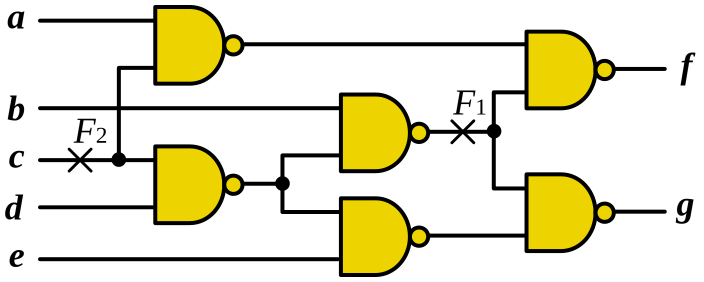
\includegraphics[width=0.7\columnwidth]{fig_c17_tf_trax}
\caption{Contrasting fault-effect propagation for the TF and TRAX models.}
\label{fig:intro_c17_tf_trax}
\end{figure}
\begin{table}[hbtp]
\renewcommand{\arraystretch}{1.2}% increase table row spacing
\centering
\begin{tabular*}{0.7\columnwidth}{@{\extracolsep{\fill}}r|r|r|c|c|c}
Fault&Fault&Two-vector test&\multicolumn{3}{c}{Output: $f g$}\\
site&type&($v_1$, $v_2$): $a b c d e$&FF&TF&TRAX\\
\hline
\multirow{2}{*}{$F_1$}&\multirow{2}{*}{STF} &$v_1: 10100$&10&10&10\\
                      &                     &$v_2: 11100$&11&10&1X\\
\hline
\multirow{2}{*}{$F_2$}&\multirow{2}{*}{STR} &$v_1: 11010$&11&11&11\\
                      &                     &$v_2: 11110$&10&11&XX\\
\end{tabular*}
\caption{Fault-free (FF) behavior of benchmark circuit c17~\cite{brglez85} (Figure~\ref{fig:intro_c17_tf_trax}) compared to TF and TRAX faults located at sites $F_1$ and $F_2$.}
\label{table:intro_tf_trax_comparison}
\end{table}
%\vskip 0.2em%

To contrast the TF and TRAX fault models, the ISCAS85 benchmark circuit c17~\cite{brglez85} is used (Figure~\ref{fig:intro_c17_tf_trax}).
%
Fault simulation is performed for TF and TRAX faults at sites $F_1$ and $F_2$, using two test-vector pairs.
%
The results of fault-effect propagation from each fault site to the circuit outputs are shown in Table~\ref{table:intro_tf_trax_comparison}.
%
The first pair of vectors activates a slow-to-fall fault at $F_1$; both the TF and TRAX produce a faulty value at output $g$.
%
In this case, both faults are detected at output $g$.
%
The second pair of vectors activates a slow-to-rise fault at $F_2$, which activates more-complex behavior and shows the difference in fault-effect propagation between TF and TRAX faults.
%
The reconvergent fanout logically masks the fault effects reaching the upper output $f$ for TF.
%
However, masking is not possible for TRAX, and both outputs take on \textit{X} values, subsuming the response of the TF.
%
The two observed \textit{X} values indicate it is possible that the actual response of a delay defect could subsume, match, or mismatch the TF response.

Since this fault model is designed to be used for diagnosis as part of a fault dictionary, attention must be paid to the computational requirements of generating such a dictionary.
%
Generating a fault dictionary using even the simplest fault model (e.g., single stuck-at) is a challenging task.
%
The task is even more daunting when using the TRAX fault model.
%
The difficulty in generating a fault dictionary is due to several factors, most notably that every fault must be simulated for all test patterns.
%
Unlike conventional fault simulation for test set evaluation, where faults are ``dropped'' after the first detection, fault dictionary generation requires full simulation results with no dropping.
%
Moreover, the complex characteristics of the TRAX fault model exacerbate the fault simulation process.
%
For example, the generalized activation conditions for the TRAX fault model involving hazards increases the complexity of fault simulation itself which means, of course, the non-dropping simulation of TRAX faults is more compute intensive.
%
As discussed later, TRAX fault simulation uses additional logic values (notably, \textit{X} and \textit{H}), which require additional memory and computation time for each gate evaluation.
%
Furthermore, the use of these additional logic values requires a complete TRAX simulation, that is, it is not possible to use the results of a simpler and faster 0/1 circuit simulator as a starting point for TRAX fault simulation.

Past efforts to accelerate fault simulation are focused around simulating in parallel and are divided into a few broad categories based on which aspect of computation is parallelized.
%
These include algorithm-parallel (\cite{agrawal87, amin97}), model-parallel (\cite{tai93, narayanan92}), and data-parallel (\cite{beece88, ozguner88, pfister82}) techniques.
%
The data-parallel techniques are further divided into fault-parallel and pattern-parallel (\cite{gulati09, parkes95, lee91}) approaches.
%
The approach presented in this work to accelerate fault simulation using GPUs uses both fault-parallel and pattern-parallel approaches for different parts of the computation.

While originally designed to speed up the highly-parallel workloads associated with 3D graphics rendering, GPUs have found new utility in the realm of high-performance parallel processing for certain types of problems, particularly for EDA-type problems~\cite{croix09}.
%
A key characteristic of the 3D graphics problem, and many other problems including fault simulation, is that very many independent calculations can be performed in parallel.
%
For example, the individual pixels of a rendered image, or the two-vector tests applied to a faulty circuit, can all be independently computed in parallel.

Although the use of GPU in EDA is relatively new, there are many publications on its use in fault simulation (\cite{gulati09, parkes95, li10, kochte10, huaweili10, gulati08, chatterjee09}).
%
All of this past work has been focused, of course, on exploiting the inherent parallelism exhibited by fault simulation.
%
What is different about the work here for dictionary construction includes the specific focus on the TRAX fault model, efficiently simulating two-vector tests, as well as various optimizations (two-input gates, a power-of-two number of logic values, etc.) targeting the specific fault simulation needs for compact dictionary generation.
%
Experiments involving various circuits, including the OpenSPARC T2 processor, demonstrate an average speed-up of nearly 8x.


\section{Hierarchical Fault Dictionary}
\label{sec:intro_dict}

In addition to the TRAX fault model, this dissertation also introduces a fault dictionary scheme optimized for performing on-chip diagnosis only to the required level of localization.
%
As previously mentioned, the only action available to an SoC at runtime is to repair, replace, or avoid a faulty module.
%
Therefore the fault dictionary needs only localize any failure(s) to the module level of the design hierarchy, hence our use of the term \textit{hierarchical fault dictionary}.

A fault dictionary for a given circuit can be conveniently viewed as a table of expected circuit responses (or some subset of the circuit response), with one row for each fault and one column for each test.
%
Each table entry is the response (or some subset) of the corresponding fault/test pair.
%
A \textit{full-response dictionary} contains the full response for each fault/test pair.
%
This dictionary can require significant storage space for modern designs.
%
As an example, the OpenSPARC T2 L2 cache write-back buffer uncore (called L2B)~\cite{sun11} contains just over 12,000 gates and uses 90 test vector pairs for test and diagnosis.
%
The full-response fault dictionary for L2B requires over 600 megabytes of storage, which is impractical for on-chip diagnosis for this relatively small circuit.
%
A variety of compaction schemes (\cite{arslan02, bernardi06, boppana94, chakravarty99, boppana96, chess99, hong07, pomeranz92}) have been developed to reduce the size of a fault dictionary, but existing schemes do not enable a sufficient level of compaction for modern designs (\cite{ryan93, boppana94}).

The TRAX hierarchical dictionary employs several techniques to reduce dictionary size.
%
First, one straightforward compaction technique is to include only faults relating to the targeted defect model (i.e., early-life and wear-out defects).
%
To this end, the TRAX fault dictionary only includes faults located at standard-cell outputs because early-life and wear-out defects affect the delay of standard cells.
%
Elimination of the remaining faults (i.e., faults located at primary inputs or fanout branches) reduces dictionary size through the elimination of dictionary rows.
%
Second, given that the system resources for on-chip test and diagnosis are necessarily limited by integrated circuit area and power budgets, it is not feasible to store the entire circuit response of every fault for every test.
%
Instead, a single bit that indicates the pass/fail outcome of a test is stored for each fault/test pair, resulting in a \textit{pass-fail dictionary}, a well-known technique for significantly reducing dictionary size at the expense of diagnostic resolution~\cite{pomeranz92}.
%
Finally, for on-chip test and diagnosis, the tested circuit (SoC core or uncore) is assumed to be partitioned into a set of modules, each of which can be independently repaired, replaced, or avoided if found to be faulty.
%
Figure~\ref{fig:intro_core_uncore_modules_faults} shows an example SoC containing three cores/uncores which themselves are composed of multiple modules, each containing TRAX faults (shown as circles within each module).
%
By recognizing that the on-chip diagnosis requirements only require fault localization to the recovery level, the diagnosis problem is significantly eased as compared to conventional approaches.

%\vskip 0.5em%
\begin{figure}[hbtp]
\centering
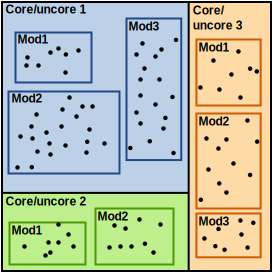
\includegraphics[width=0.4\columnwidth]{fig_core_uncore_modules_faults}
\caption{Hierarchical view of a system-on-chip (SoC) that contains multiple cores and uncores, each of which contain multiple modules.
%
Each module contains a number of faults.}
\label{fig:intro_core_uncore_modules_faults}
\end{figure}
%\vskip 0.5em%

Given this relaxation of diagnosis requirements, the concept of intra- and inter-module fault sets can lead to significant reduction in the fault count (and therefore dictionary size) necessary for accurate diagnosis.
%
For faults within the same module that are test-set equivalent (that is, those having equivalent simulation responses for all tests), all but one can be eliminated from the dictionary, as distinguishing them is unnecessary for determining a defective module.
%
Another technique to eliminate intra-module faults is called \textit{subsumption}, which is similar to the traditional concept of fault dominance, but is subtly different.
%
In brief, using the TRAX fault model and hierarchical dictionary scheme enables the elimination of any fault with a response that is subsumed by another fault in the same module.
%
A subsumed fault is no longer needed because if it fails, it would still be accurately represented in the dictionary by the subsuming fault.

%\vskip 0.5em%
\begin{table}[hbtp]
\centering
\begin{tabular*}{0.9\columnwidth}{@{\extracolsep{\fill}}cccccccl}
\toprule
Fault&Module&$T_1$&$T_2$&$T_3$&$T_4$&$T_5$&\\
\midrule
$F_1$&$M_1$&P&F&F&P&F&\\
$F_2$&$M_1$&P&F&F&P&F&Eliminated (EQU)\\
$F_3$&$M_1$&P&F&P&P&P&Eliminated (SUB)\\
$F_4$&$M_1$&F&F&P&P&F&\\
\midrule
$F_5$&$M_2$&F&F&P&P&F&\\
$F_6$&$M_2$&P&P&F&F&P&\\
\bottomrule
\end{tabular*}
\caption{TRAX fault dictionary data illustrates dictionary compaction, using equivalence and subsumption relationships to eliminate two intra-module faults.}
\label{table:intro_fault_resp}
\end{table}
%\vskip 0.2em%

Table~\ref{table:intro_fault_resp} shows an example of equivalence and subsumption fault reduction, where fault $F_2$ is eliminated via equivalence to $F_1$, and $F_3$ is eliminated because it is subsumed by both $F_1$ and $F_4$.
%
These two techniques for fault reduction are only applied to faults belonging to the same module, because repair-level diagnosis does not require distinguishing intra-module faults.
%
Applying these dictionary compaction techniques produces a \textit{collapsed pass/fail hierarchical dictionary}, which is used in the diagnosis experiments presented later.
%
For the L2B fault dictionary mentioned before, the full-response dictionary of over 600 megabytes is compacted to less than 32 kilobytes for the collapsed pass/fail dictionary, which is a reduction of over 20,000X.


\section{On-Chip Diagnosis Architecture}
\label{sec:intro_diag}

On-chip test and diagnosis using TRAX faults assume deployment of CASP (Concurrent Autonomous chip self-test using Stored Patterns)~\cite{li08}.
%
In CASP, a small amount of extra hardware is added to the chip to allow for the re-use of DFT logic for in-field test of the chip.
%
High-quality test vectors are stored in off-chip memory and are periodically loaded into the chip one vector at a time for test application and response observation.
%
The CASP process consists of four phases.
%
First, the CASP controller selects an SoC core/uncore for test.
%
Second, the selected core/uncore is taken offline and isolated from the rest of the system.
%
Third, each test is loaded from off-chip memory and applied to the isolated core/uncore, re-using existing design-for-test (DFT) scan logic.
%
Finally, once all tests are applied, the CASP controller returns the core/uncore to normal operation.
%
The recorded test responses are then provided to the on-chip diagnosis architecture for analysis and fault localization.
%
Since each core/uncore is tested and diagnosed independently, each type of core/uncore requires a separate fault dictionary, and a single dictionary is shared by each duplicated core/uncore.

The objective of on-chip diagnosis is to determine which module(s) of the core/uncore are defective, based on the observed test failures.
%
Due to the inherent nature of on-chip diagnosis, existing off-line approaches for multiple-defect diagnosis~\cite{pomeranz16,yu10,chen14} are not directly applicable.
%
Here, the previously-described TRAX hierarchical fault dictionary is used, which stores a single bit for each fault-test pair, indicating if the corresponding fault is detected by the corresponding test.
%
The TRAX dictionary is used in conjunction with the pass/fail test response to produce a list of potentially responsible ``candidate'' faults.
%
Specifically, starting with a list of all TRAX faults within the tested core/uncore dictionary, each failing test response is used one at a time to eliminate any faults that are not detectable by that failing test.
%
This is an instance of Tester-Fail/Simulation-Pass (TFSP) and triggers the elimination of the corresponding fault.
%
After all test responses are processed, what remains is a list of candidate TRAX faults compatible with the observed behavior.

Each fault in the list of candidate TRAX faults belongs to a specific hierarchal module of the core/uncore.
%
The candidate fault list is analyzed to count the number of candidate faults belonging to each module, resulting in a per-module candidate fault count.
%
These fault counts are used to determine which module or modules are likely defective.

A scalable on-chip diagnosis architecture is developed to use the hierarchical dictionary to localize failures only to the required level.
%
Diagnosis hardware scaled to the size of one of the largest analyzed circuits, NCU from the OpenSPARC T2 design, requires between 22,000 - 26,000 clock cycles (depending on the desired scaling) for performing diagnosis.
%
Hardware requirements range between 38,000 - 245,000 additional gates, corresponding to between 0.0077\% - 0.0491\% estimated area overhead.

\section{Multiple Defect Diagnosis}
\label{sec:intro_multi}

The TRAX fault model is designed to capture the arbitrary slowdown exhibited by a single early-life or wear-out failure.
%
Due to the very nature of the targeted failures, it is likely however that more than one failure will be present.
%
Given the conservative propagation properties of the unknown value \textit{X}, the use of the TRAX-based hierarchical dictionary can remain effective even in the presence of multiple faults.
%
This is particularly the case in the context of the targeted failure modes (early-life and wear-out failures) and the relaxed diagnostic requirements (fault localization only to the recovery level).

In Chapter~\ref{chap:multi}, an empirical analysis is performed to determine the effectiveness of the TRAX-based hierarchical fault dictionary for on-chip diagnosis, when faced with multiple runtime failures.

\section{Benchmark and Test Circuits}
\label{sec:intro_benchmark_and_test_circuits}

Measuring dictionary size reduction due to fault elimination requires access to designs that exhibit module-level hierarchy.
%
The hierarchical versions of the ISCAS85 benchmark circuits~\cite{brglez85} produced by the University of Michigan~\cite{hansen99} serve this purpose well since many of the benchmarks have been reverse engineered to at least two levels of hierarchy.
%
Additionally, three other circuit sources are utilized.
%
First, several circuits are taken from the ITC99 benchmark set~\cite{corno99}.
%
Second, two sub-circuits are taken from the freely-available OpenSPARC T2 processor design~\cite{sun11}, the previously-mentioned L2 cache write-back buffer uncore (L2B), and the Non-Cachable Unit (NCU) that decodes and directs I/O addresses.
%
Third, five circuits are taken from the EPFL combinational benchmarks suite~\cite{epfl}.
%
The non-ISCAS circuits are not pre-partitioned into a module-level hierarchy and are instead partitioned into ten modules using graph clustering and partitioning software~\cite{dhillon07}.
%
In our experiments, we equate the second-level modules of the circuits to the level of repair.
%
In other words, diagnostic precision has to be only achieved at the second level of the hierarchy within these circuits.
%
Details of the test patterns generated using a commercial ATPG tool are shown in Table~\ref{table:intro_circuit_details}.
%
As it does not support the TRAX fault model, the commercial ATPG tool is configured to generate test vector pairs targeting the transition fault (TF) model.
%
As will be explained in Chapter~\ref{chap:trax}, the activation conditions of a TRAX fault are a superset of the activation conditions of a transition fault, meaning that ATPG targeting transition faults produces a test set also effective at detecting TRAX faults.

%\vskip 0.5em%
\begin{table}[hbtp]
\center
\begin{tabular*}{0.8\columnwidth}{@{\extracolsep{\fill}}rrrr}
\toprule
Benchmark   &Transition faults     &Test pairs &Fault coverage\\
\midrule
c432        &316        &37         &99.05\%\\
c499        &456        &71         &100.00\%\\
c1355       &1,028      &106        &99.51\%\\
c1908       &578        &64         &99.65\%\\
c2670       &1,996      &67         &96.69\%\\
c3540       &2,674      &128        &99.25\%\\
c5315       &4,308      &85         &100.00\%\\
c7552       &5,530      &84         &98.63\%\\
\midrule
b12         &1,880      &80         &100.00\%\\
b14\_opt    &10,694     &345        &99.97\%\\
b14         &19,534     &657        &99.67\%\\
b15         &16,734     &407        &97.39\%\\
b17\_opt    &45,514     &600        &98.38\%\\
b18\_opt    &139,826    &704        &99.71\%\\
b22         &59,568     &554        &99.69\%\\
\midrule
L2B         &24,444     &90         &99.99\%\\
NCU         &67,124     &211        &99.95\%\\
\midrule
epflDiv     &203,206    &612        &99.25\%\\
epflMult    &101,008    &77         &99.96\%\\
epflSqrt    &82.084     &161        &91.91\%\\
epflSquare  &70,984     &79         &100.00\%\\
epflMemCtrl &165,076    &1,276      &99.84\%\\
\bottomrule
\end{tabular*}
\caption{ATPG details for benchmark circuits, including the number of transition faults, number of test pairs, and fault coverage.}
\label{table:intro_circuit_details}
\end{table}
%\vskip 0.5em%


\section{Dissertation Organization}
\label{sec:intro_dissertation_organization}


The rest of this dissertation is organized as follows: Chapter~\ref{chap:trax} details the TRAX fault model, including comparisons with existing fault models.
%
Chapter~\ref{chap:trax} also describes the GPU-accelerated fault simulator developed for specifically simulating TRAX faults in an efficient manner.
%
Chapter~\ref{chap:dict} describes the hierarchical dictionary and investigates its performance for a variety of benchmark circuits.
%
The on-chip fault diagnosis architecture is detailed in Chapter~\ref{chap:diag}.
%
The combination of the TRAX fault model, hierarchical dictionary, and on-chip diagnosis architecture is also evaluated in Chapter~\ref{chap:diag} using defect injection and diagnosis experiments.
%
Chapter~\ref{chap:multi} evaluates the efficacy of on-chip diagnosis for multiple injected defects.
%
Finally, Chapter~\ref{chap:conclusions} concludes the dissertation and includes direction for future work.

\chapter{TRAX Fault Model}
\label{chap:trax}

In the context of digital circuit testing, a fault model is an abstraction of a class of defects, created to simplify their characteristics in order to make analysis more tractable.
%
Fault models are particularly useful for understanding the high-level impact of a defect on circuit behavior.
%
The simplest fault model, the single stuck-line (SSL) model~\cite{abramovici90}, assumes each individual signal line is susceptible to becoming permanently stuck at either logic-low or logic-high.
%
Another fault model, the bridge fault model~\cite{abramovici90}, hypothesizes that two signals are errantly connected.
%
Depending on the relative drive strengths of the two bridged signals the stronger may override the weaker, or the two signals may form a wired-AND or wired-OR logic function.

The choice of fault model is largely a tradeoff between how closely a fault model matches the targeted defects and the size of the fault universe.
%
Simpler fault models such as the SSL have a relatively small fault universe ($2 n$, where $n$ is the number of circuit signal lines), while more complex fault models like the bridge model have a larger fault universe (for $m$-line bridges, on the order of $m^n$i, in theory).
%
In general, the preferred fault model for any particular situation is the fault model that best captures the expected effects of the targeted defects while still having a sufficiently small fault universe.

In this thesis, the targeted defects are early-life and wear-out failures.
%
Early-Life Failures (ELF) are caused by latent manufacturing defects not detected by factory tests, such as gate-oxide defects~\cite{chen08}.
%
Chips affected by ELF can fail early in their lifetime, often much sooner than the specified product lifetime.
%
ELF-affected transistors will experience gradual delay increases over time before functional failures occur.
%
Wear-out failures include mechanisms like Negative Bias Temperature Instability (NBTI), which changes the threshold voltage of a PMOS transistor, resulting in decreased transistor drive current, ultimately leading to circuit-speed degredation~\cite{borkar06,schroder03}.
%
NBTI first became a significant issue at the 90nm technology node~\cite{agarwal07} but worsens as technology continues to scale~\cite{reddy02}.
%
Various experiments involving actual test chips~\cite{agarwal07,chen09} demonstrate that both early-life and wear-out failures manifest as delay increases in standard cells.

\section{Existing Fault Models}
\label{sec:trax_existing_fault_models}

There are a variety of fault models targeting changes in circuit delays, such as those caused by early-life and wear-out failures.
%
For example, the path delay fault model~\cite{smith85,lin87} characterizes a delay-causing defect as an accumulation of additional path delay through the circuit from a primary input to a primary output.
%
This model, however, suffers from the fact that the number of path-delay faults can be exponential in the number of circuit lines~\cite{heragu96}, leading to a large fault universe.
%
The segment delay fault model~\cite{heragu96}, on the other hand, is a parameterized fault model that models delay as distributed along a short segment (of length $L$) of a path, where the parameter $L$ is chosen based on defect statistics.
%
The size of the fault universe can be controlled by the choice of $L$.
%
Other delay fault modules include the Transition Path Delay Fault model~\cite{pomeranz08tpdf}, the Propagation Delay Fault model~\cite{lin05}, and the Inline Resistance Delay Fault model~\cite{benware04}.
%
An ideal fault model to represent the slowdown caused by early-life and wear-out failures is the gate delay fault (GDF) model~\cite{jha03}.
%
Detection of a GDF requires producing a transition at the affected gate output and sensitizing a circuit path from the gate to one or more primary outputs.
%
A GDF will only be detected if the additional delay due to the fault is larger than the slack of a path appropriately sensitized.
%
Identifying a test to detect a GDF is thus an optimization problem that involves searching for a sensitizable path through the gate that exhibits the minimal slack.
%
Optimization adds undesired complexity to the already intractable test generation process, making deployment of the GDF model for use in a dictionary much more challenging.

The most commonly-deployed delay fault model is the transition fault (TF) model~\cite{jha03}.
%
It is widely used because it is a delay fault model with a limited fault universe and very related to the ubiquitous SSL fault model~\cite{wang14}.
%
Whereas the GDF model makes no assumption about the increase in delay, the TF model, on the other hand, assumes the delay to be larger than the slack of any sensitized path through the fault site.
%
This assumption significantly reduces complexity because any test that sensitizes a path from the fault site to an observable point will detect a TF fault.
%
That is, test generation remains a satisfiability problem as opposed to an optimization problem.
%
The TF model is more tractable but is very pessimistic since it implicitly assumes that every fault will produce errors at the output of each sensitized path.%todo add wang14 to intro trax section

The unspecified-transition fault (UTF) model~\cite{pomeranz08} is a compromise between the gate delay fault model and the transition fault model.
%
The UTF model makes no assumptions about the length of the delay and represents the uncertainty in fault delay through the use of the unknown value \textit{X}, produced when a UTF is activated.
%
While the GDF model makes no assumptions about delay size, and the TF model assumes a worst-case gross delay, the UTF exists as a compromise, using the \textit{X} value to represent the uncertainty of the modeled delay.
%
This chapter of the dissertation details an enhancement of the UTF model that includes activation and propagation due to glitches resulting from hazards, noise\footnote{Due to limitations in the gate-level Verilog simulations used to generate circuit responses from injected delays, we do not consider noise-based activation.}, etc.
%
We refer to this new fault model as the Transition-X (TRAX) fault model.

\section{TRAX Fault Model}
\label{sec:trax_trax}

Similar to a transition fault, a TRAX fault is either a slow-to-fall (STF) or slow-to-rise (STR) fault, and is activated by either a transition of the correct polarity (1-to-0 or 0-to-1, respectively) or due to a glitch.
%
Activation-by-glitch is the prime difference between the TRAX and the unspecified-transition fault models.
%
Simulation experiments (designed to mimic slow-downs due to aging) revealed that some failing responses could not be explained by any UTF.
%
Further investigation revealed the source of this discrepancy, namely that signal glitches activated the injected rising or falling delays.
%
This situation is not covered by the conventional transition-based fault activation used by TF and UTF, and the TRAX fault model is developed to also include glitch-based fault activation.
%
This enhancement ensures that TRAX fault effects subsume the effects of a co-located delay defect.

A glitch is an undesired and transient pulse in a signal, typically generated at the output of a gate driven by two successive sets of inputs that do not provide a constant controlling input\footnote{A glitch can also be created by excessive noise in cross-coupled on-chip interconnects~\cite{cuviello99}, but noise is not considered in this work due to limitations of the gate-level Verilog simulation employed.}.
%
To explain this concept further, we first need some background:

\begin{itemize}
\item In the two-vector test scheme employed in this work, each test consists of two test vectors, referred to as $V_1$ and $V_2$.
\item Many gate types have a ``controlling input'' that forces the gate output to a certain value regardless of the other gate inputs.
%
For example, the controlling input value for a NAND gate is logic-low; any low input will force the gate output high.
%
XOR and XNOR gates do not have a controlling input value.
\item A controlling input is ``constant'' if at least one of the gate inputs is driven with a constant controlling value in both $V_1$ and $V_2$.
\end{itemize}

For a two-input NAND gate $Y = \overline{(A \land B)}$, the inputs ($A = 0 \rightarrow 0$, $B = 1 \rightarrow 0$) provide a constant controlling value (logic-low) to input $A$, leading to a constant gate output of ($Y = 0 \rightarrow 0$).
%
In contrast, for the inputs ($A = 0 \rightarrow 1$, $B = 1 \rightarrow 0$), even though the expected output is also ($Y = 0 \rightarrow 0$), there exists the potential of a gate output glitch ($Y = 0 \rightarrow 1 \rightarrow 0$) due to the lack of a constant controlling input.
%
Such a test pair, with no constant controlling input, is referred to as a \textit{hazardous} test pair, given the potential for a glitch on the gate output.
%
In the TRAX fault model, where all faults are placed at gate outputs, a fault can be activated by a glitch due to a coincident hazard.
%
The hazard condition is added as a fourth logic value for TRAX fault simulation, resulting in a four-valued algebra of \verb+{0, 1, X, H}+.
%
The extended truth tables for the eight primitive gates are shown in Figure~\ref{fig:trax_gate_evaluation}.

%\vskip 0.5em%
\begin{figure}[htbp]
\centering
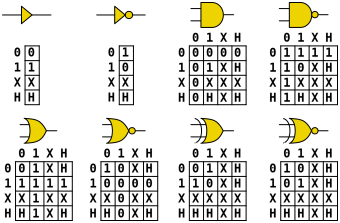
\includegraphics[width=0.8\columnwidth]{fig_gate_evaluation}
\caption{Truth tables for the eight primitive gate types are extended to support the four-value logic of the TRAX fault model.}
\label{fig:trax_gate_evaluation}
\end{figure}
%\vskip 0.5em%

An advantage of the TRAX fault model is that the \textit{X} value captures all the possible transport-delay changes that can be exhibited by a gate affected by NBTI or ELF since the propagation of the \textit{X} value is conservative.
%
Whereas the errors from a conventional transition fault could interact to either increase or reduce the number of fault-effect observations (i.e., failing outputs), the use of the \textit{X} value can only increase the number of failing outputs.
%
In other words, the set of sensitized paths with \textit{X} values will subsume the sensitized paths associated with any GDF of any delay.
%
In addition, any error cancelling due to fault masking that may occur due to the TF fault model is not possible in the TRAX fault model.

The ISCAS85 benchmark circuit c17 \cite{brglez85} shown in Figure~\ref{fig:trax_c17_tf_trax} is used to contrast the TF and TRAX models.
%
TF and TRAX faults are simulated at both sites $F_1$ and $F_2$, using two test-vector tests.
%
Table~\ref{table:trax_tf_trax_comparison} shows how fault effects propagate from each fault site to the circuit outputs.
%
The first pair of vectors activates a slow-to-fall fault at $F_1$; both the TF and TRAX produce a faulty value on the lower output $g$.
%
For this case, both faults are detected and produce the same response.
%
The second pair of vectors activates a slow-to-rise fault at $F_2$.
%
Here, more complex behavior arises, demonstrating the difference between TF and TRAX.
%
For TF, the reconvergent fanout logically masks the slowed transitions reaching the upper output $f$.
%
Masking is not possible for TRAX, resulting in both outputs having \textit{X} values, which subsumes the response of the TF.
%
The \textit{X} values at the two outputs mean it is possible that the actual response of a slowdown could subsume, match, or mismatch the TF response.

%\vskip 0.2em%
\begin{figure}[hbtp]
\centering
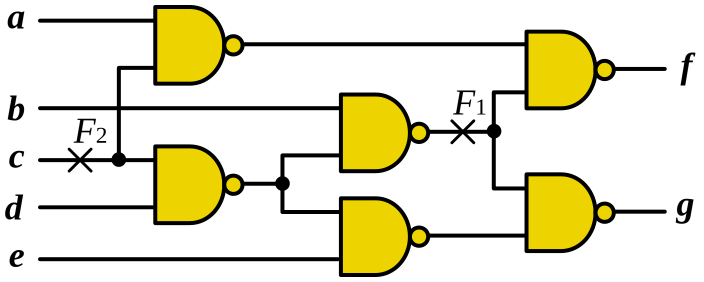
\includegraphics[width=0.8\columnwidth]{fig_c17_tf_trax}
\caption{Contrasting fault-effect propagation for the TF and TRAX models.}
\label{fig:trax_c17_tf_trax}
\end{figure}
\begin{table}[htbp]
\renewcommand{\arraystretch}{1.3}% increase table row spacing, adjust to taste
\centering
\begin{tabular*}{0.9\columnwidth}{@{\extracolsep{\fill}}r|r|r|c|c|c}
Fault&Fault&Two-vector test&\multicolumn{3}{c}{Output: $f g$}\\
site&type&($v_1$, $v_2$): $a b c d e$&FF&TF&TRAX\\
\hline
\multirow{2}{*}{$F_1$}&\multirow{2}{*}{STF} &$v_1: 10100$&10&10&10\\
                      &                     &$v_2: 11100$&11&10&1X\\
\hline
\multirow{2}{*}{$F_2$}&\multirow{2}{*}{STR} &$v_1: 11010$&11&11&11\\
                      &                     &$v_2: 11110$&10&11&XX\\
\end{tabular*}
\caption{Fault-free (FF) behavior of benchmark circuit c17 \cite{brglez85} (Figure~\ref{fig:trax_c17_tf_trax}) compared to TF and TRAX faults located at sites $F_1$ and $F_2$.}
\label{table:trax_tf_trax_comparison}
\end{table}
%\vskip 0.2em%

Fault simulation of TRAX faults is very similar to the TF model.
%
Instead of assuming a grossly-slowed transition, an \textit{X} value is injected when a TRAX fault is activated, either by a conventional transition or by a hazard value.
%
These injected \textit{X} values are propagated through the simulated circuit, producing the fault-free values of 0, 1, or the potentially faulty value \textit{X} at the observation points.
%
Additionally, a TRAX-without-hazards fault model variant (which is equivalent to the UTF model), where a fault can only be activated by a conventional transition, is also used in later sections to evaluate fault dictionary size (Section~\ref{sec:dict_exp_size_res}) and on-chip diagnosis effectiveness (Section~\ref{sec:diag_exp_traxnh}).

Interpretation of observed \textit{X} values at the outputs of the circuit under test requires further discussion.
%
Observed \textit{X} values resulting from TRAX fault simulation identify outputs that could, but not necessarily, be affected by a slowdown at the fault site.
%
In other words, outputs that have \textit{X} values may or may not exhibit an error, depending on the level of slowdown.
%
It is assumed for every test that detects a given TRAX fault that at least one observed \textit{X} value will actually be erroneous, guaranteeing detection.
%
Since no knowledge about the timing is assumed, it cannot be known a priori however which output will take on an incorrect value when a TRAX fault is detected.
%
Due to this uncertainty, the set of potentially-faulty outputs for a particular fault-test pair tells a different tale than the fault simulation responses of a conventional fault model.
%
For example, the fault simulation output for a particular transition fault describes how the circuit would behave if it were affected by a gross-delay defect located at the same point in the circuit as the modeled fault.
%
In contrast, the uncertainty as to which TRAX potentially-faulty outputs actually produce a faulty output means that it does not describe the expected response of a co-located defect.
%
Instead, the set of potentially-faulty outputs for a TRAX fault-test pair describes which circuit outputs \textit{could} be affected by a co-located defect.
%
This is a subtle point that supports the general-purpose nature of the TRAX fault model.
%
Effectively, TRAX fault simulation captures the relationship between incorrect circuit outputs and the set of modeled TRAX faults that could have caused that faulty behavior.
%
This enables TRAX to handle not just defects that increase delay, but also defects that decrease delay.


\section{GPU-Accelerated TRAX Fault Simulation}
\label{sec:trax_gpu}

The task of generating a fault dictionary is a challenge, even using the simplest fault model (e.g., single stuck-at).
%
The most notable factor is that every fault must be simulated for all test patterns.
%
While conventional fault simulation for test set evaluation can ``drop'' faults after each is first detected, dropping is not possible for a full fault dictionary generation because it requires full simulation results to form each entry of the full dictionary table.

The fault simulation process is exacerbated by the complex characteristics of the TRAX fault model.
%
The generalized activation conditions for a TRAX fault (for example, the previously mentioned hazard generation and associated fault activation), increase the complexity of fault simulation itself, meaning of course that the non-dropping simulation of TRAX faults is computationally more intensive.
%
As previously discussed, TRAX fault simulation uses two additional logic values beyond the customary 0 and 1, (that is, \textit{X} and \textit{H}).
%
A larger set of logic values requires additional memory and computation time for the evaluation of each gate.
%
Compounding this is the fact that the use of these additional logic values requires a complete TRAX simulation, that is, we cannot simply use the results of a simpler and faster 0/1 circuit simulation as a starting point for TRAX fault simulation.

Past efforts to accelerate fault simulation can be divided into a few categories, including algorithm-parallel (\cite{agrawal87, amin97}), model-parallel (\cite{tai93, narayanan92}), and data-parallel (\cite{beece88, ozguner88, pfister82}) techniques.
%
Data-parallel techniques are further divided into fault-parallel and pattern-parallel approaches (\cite{gulati09, parkes95, lee91}).
%
Both fault- and pattern-parallel approaches are used in this work (at different phases of the computation) to accelerate fault simulation using Graphics Processing Units (GPUs).

While originally designed to accelerate the highly-parallel workloads associated with 3D graphics rendering, GPUs have found new utility in high-performance parallel processing for certain types of problems, particularly for EDA-type problems~\cite{croix09}.
%
A key characteristic of the 3D graphics problem, and many other problems including fault simulation, is the large number of independent calculations (individual pixels of a rendered image, and the independent two-vector tests applied to a faulty circuit, for example).

Although the use of GPU in EDA is relatively new, there are a number of publications on its use in fault simulation (\cite{gulati09, parkes95, li10, kochte10, huaweili10, gulati08, chatterjee09}).
%
All of this past work has been focused on exploiting the inherent parallelism of the fault simulation problem.
%
Unique aspects of the GPU-accelerated dictionary construction presented here includes the specific focus on the TRAX fault model, efficiently simulating two-vector tests, as well as a few interesting optimizations (two-input gates, a power-of-two number of logic values, etc.) targeting the specific fault simulation needs for compact dictionary generation.
%
Details about the unique features of the fault simulator are provided in the following sub-sections.

\subsection{GPU Architecture and CUDA Programming Model}
\label{sec:trax_gpu_arch_cuda}
In 2006, NVIDIA introduced the CUDA (Compute Unified Device Architecture)~\cite{cuda} GPU architecture and programming interface.
%
CUDA acts as an extension to existing C/C++ programs, enabling the use of the GPU as a co-processor for executing highly-parallel workloads, without having to remap computations into a graphics language such as OpenGL~\cite{opengl}.
%
In the CUDA architecture, the GPU acts as a specialized accelerator or co-processor, accessed by C/C++ language extensions.
%
By using special function calls, the CPU code can schedule and execute a ``Kernel'' of code on the GPU, as well as transfer data between CPU memory and GPU memory.

Each GPU consists of a varying number of streaming multiprocessors (SMs), each composed of multiple CUDA cores (ALUs).
%
Each core of an SM executes the same instruction in every clock cycle but can operate on different data, commonly called a Single Instruction Multiple Data (SIMD) architecture.
%
If the cores of an SM execute a data-dependent branch instruction and choose different paths (so-called \textit{branch divergence}), the SM must split the cores into multiple groups and execute each group serially, drastically reducing overall performance.

The GPU includes a variety of memory types.
%
The largest memory is the global device memory, which is read/write (but not cached), and is on the order of gigabytes.
%
Access to global memory has high bandwidth but very long latency and can be several hundred clock cycles in delay.
%
Fortunately, this latency can be typically hidden through aggressive thread swapping (provided there are sufficient arithmetic operations pending).
%
Multiple global memory accesses from different threads can coalesce together into a single memory request, but only if the accesses are properly aligned and distributed into memory transactions of size 32-, 64-, or 128-bits.
%
In addition to global device memory, each SM in the GPU contains shared memory that is accessible by all threads in the current thread block, frequently used when threads need to access the same data as their neighboring threads.
%
At the lowest level, the GPU has a pool of several thousand registers available for private use by active threads.
%
All of these memories are read/write and are not cached, but there also exist two types of read-only, cached memory, which are the \textit{texture} and \textit{constants} memory.
%
Texture memory is special in that its caching is optimized for two-dimensional spatial locality.

The threads of a CUDA program are organized into a hierarchy consisting of threads, warps, blocks, and grids.
%
Threads are the smallest unit of computation and are organized into \textit{warps} (the smallest schedulable unit of threads, guaranteed to all run on the same SM), which can coordinate their execution through the use of fast shared memory and block-level synchronization operations.
%
Warps are collected into blocks, which are further collected into a \textit{grid} of threads, which encompasses the entire execution structure of a given CUDA kernel.
%
Warps are used to hide the long latency of global memory by quickly swapping-out any warp waiting for a memory transfer.

\subsection{Fast Fault Simulation Approach}
\label{sec:trax_gpu_approach}
The specialized hardware of a GPU enables high-performance execution of highly-parallel workloads, but care must be taken to design the memory structures and GPU kernel code to gain the greatest possible advantage of the available hardware.
%
Our approach to GPU-accelerated TRAX fault simulation is organized into three distinct phases of operation, performing either pattern-parallel or fault-parallel processing:

\begin{enumerate}
\item Perform a fault-free simulation for each two-vector test
\item Determine which tests activate each fault
\item Perform fault simulation for each fault activation
\end{enumerate}

These three phases directly correspond to the three GPU kernels developed in this work and explained in the following subsections.
%
However, a few issues regarding the GPU fault simulator should be discussed first.

As previously mentioned, TRAX fault simulation uses two-vector tests, where each test consists of a pair of vectors labeled $V_1$ and $V_2$.
%
Fault simulation is focused on the creation of different ``circuit states'' using fault simulation.
%
Each test has a fault-free circuit state, recording the fault-free values for each gate and circuit input, for both $V_1$ and $V_2$.
%
Creating these fault-free circuit states for all tests is the focus of GPU Kernel 1 (details in Section~\ref{sec:trax_gpu_k1}).
%
These fault-free circuit states (one per two-vector test) are then analyzed to determine which faults are activated by each test pair (GPU Kernel 2 in Section~\ref{sec:trax_gpu_k2}).
%
Finally, GPU Kernel 3 (Section~\ref{sec:trax_gpu_k3}) updates copies of the fault-free circuit state to propagate the activated fault \textit{X} values to the circuit outputs and determines which faults are detected by which tests.

In addition to the typical zero and one logic values, the TRAX fault model also utilizes the unknown \textit{X} value and hazard values.
%
In the interest of having a power-of-two number of logic values, the hazard-0 and hazard-1 values are combined into a single hazard (\textit{H}) value.
%
This simplification does not reduce the accuracy of the fault simulation since the hazard polarity can always be determined by examining the fault-free value of the circuit at that location.
%
This leaves a four-valued algebra of \verb+{0, 1, X, H}+, which requires extending the truth tables for the eight primitive gates used in the GPU-based fault simulator as shown in Figure~\ref{fig:trax_gate_evaluation} on page~\pageref{fig:trax_gate_evaluation}.

\subsubsection{Circuit Structure Optimization}
Due to the limitations and architecture of the GPU memory and stream processors, it is beneficial to limit the types and circuit structures that can be fault simulated to improve efficiency.
%
These restrictions regularize the size of individual entities in the circuit netlist and enable a less complex and more efficient simulation process.

The first netlist restriction is that only one- or two-input gates are permitted, meaning that larger gates must be partitioned into equivalent subcircuits of smaller gates.
%
Restricting the netlist to small gates enables a simple, constant-size data structure for each gate in the circuit netlist, and increases the performance of the gate evaluation process.
%
Because the simulator requires a list of faults for simulation instead of assuming faults at every gate output, this expansion of a large gate into a set of smaller gates is not a significant barrier to the use of the fault simulator.
%
While this two-input gate restriction results in a larger number of gates, due to larger gates being split into several two-input gates, the resulting regularization of data structures and minimization of gate evaluation lookup tables results in a more efficient fault simulation process.
%
Gate size restriction is not a TRAX-specific optimization and can be implemented regardless of the chosen fault model.

Additionally, in a purely combinational circuit with no feedback, it is possible to sort the gates by level to produce a topological ordering for gate evaluation.
%
If the gates of the circuit are evaluated in topological order, it is guaranteed that the input values to each gate will have already been computed before the evaluation process reaches the gate.
%
This enables a single-pass simulation, where each gate is evaluated only once, simplifying the simulation process and increasing performance by ensuring that the memory accesses are well-aligned and progress through device memory in an orderly fashion (that is, gates and circuit states are stored within GPU memory in their topological order, eliminating the need for low-performance random memory accesses).%todo add a little diagram to illustrate topological ordering of gates? Maybe split paragraph with figure in middle before "this enables a single-pass"

\subsubsection{GPU Data Structures}
Given the SIMD architecture of the GPU hardware, it is critical to optimize the storage format and access patterns of data structures in the memory of the GPU.
%
There are two competing goals to consider in designing the data structures:

\begin{itemize}
\item Storage compactness (space efficiency)
\item Ease of access (instruction efficiency)
\end{itemize}

The approach taken with these data structures is to compact the data as much as possible in order to enable the processing of very large circuit netlists.
%
Only if profiling reveals a bottleneck in access for a given data structure will that structure be modified to improve instruction efficiency.

The first data structure is the circuit netlist, which is stored as an array of Gate structs.
%
Each Gate structure includes the gate type, a boolean flag to indicate if the gate drives a primary output, and the net index of each of the two gate inputs.
%
The gates are stored in circuit topological order, indexed by their output \verb+netID+, such that the gate that drives net 0 is stored first, the gate that drives net 1 is stored next, and so on.

The second data structure is the collected state of all the gates and primary inputs of a circuit (either the fault-free circuit or one of the many faulty circuits), which is read and written by the fault simulation kernels.
%
This circuit state is stored in a packed format, with four 2-bit logic values per byte, sorted by net index.
%
For two-vector TRAX fault simulation, two values must be stored for each net.
%
Accessing state values is still relatively simple, i.e., accessing the \verb+v1+ (vector 1) value of \verb+netID+ is simply \verb+state[netID * 2]+ and the \verb+v2+ value is accessed by \verb=state[netID * 2 + 1]=.
%
To simplify the GPU code, the gates are stored in topological order, as previously mentioned.
%
The values of the primary inputs under \verb+v1+ and \verb+v2+ are stored in the circuit-state array after all of the gates, as illustrated in Figure~\ref{fig:trax_gpu_state_structure}.
%
The PI values are stored after the gate values in order to simplify the lookup of gate output values, specifically, the output values of gate $i$ are stored in the state array at position $2 \times i$ and $2 \times i + 1$.

%\vskip 0.5em%
\begin{figure}[hbtp]
\centering
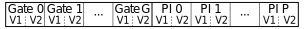
\includegraphics[width=\columnwidth]{figures/fig_gpu_state_structure.pdf}
\caption{The base data structure of GPU fault simulation is the circuit state, consisting of the $V_1$ and $V_2$ values of each gate output and primary input.
%
Each circuit state (either fault-free or faulty, for test vectors $V_1$ and $V_2$) is stored in a packed format, consisting first of the topologically-sorted gate output values, followed by the primary input values, with two bits per value.}
\label{fig:trax_gpu_state_structure}
\end{figure}
%\vskip 0.5em%

The third data structure is a lookup table for gate evaluation, a very frequent operation.
%
As previously mentioned, gates are restricted to one or two inputs, making it very simple to craft a lookup table to perform the gate evaluation.
%
The output value of a gate depends on the gate type and the two input values.
%
With eight primitive gate types (three bits) and two input values (two bits each), seven bits can be used to uniquely determine the output of a gate.
%
The gate-evaluation lookup table, therefore, contains $2^7 = 128$ values.
%
The one-input gates (the buffer and the inverter) only have four possible input combinations instead of 16, meaning that some of these values in the lookup table are redundant, but are maintained in the interest of lookup table regularity.
%
The gate-evaluation lookup table is stored in the GPU constants memory, which is a high-speed cached memory, and permits penalty-free parallel access by multiple threads.
%
The index into the lookup table is constructed from the gate type and the two input values, resulting in a seven-bit value, denoted as:

\begin{verbatim}
index = (gate.type << 4) | (in1_value << 2) | (in2_value)
\end{verbatim}

\subsubsection{Kernel 1 - Fault-Free Circuit Simulation}
\label{sec:trax_gpu_k1}

The first step of the fault simulation process is to compute the fault-free circuit states for all two-vector tests.
%
This is accomplished by Kernel 1 in the implementation, which assigns one GPU thread per test.
%
Before launching the GPU kernel, memory is first allocated to store one circuit state per test.
%
Each circuit state is then initialized with the proper test input values, with \textit{X} values assigned to all gate outputs.
%
The pseudocode of Kernel 1 is shown in Algorithm~\ref{alg:trax_gpu_k1}, and a graphical representation is shown in Figure~\ref{fig:trax_gpu_k1}.

\begin{algorithm}
\centering
\caption[GPU Kernel 1: Fault-Free Circuit Simulation]{-- Kernel 1: Fault-Free Circuit Simulation}
\label{alg:trax_gpu_k1}
\begin{algorithmic}[1]
\STATE testID = (blockID $\times$ BLOCKSIZE) + threadID
\IF{testID $<$ numTests}
  \STATE myState = allStates + (bytesPerState $\times$ testID)

  \COMMENT{iterate over all gates in topological order}
  \FOR{gateID = 0 \TO (numGates - 1)}
    \STATE cudaFaultSimCore(gates[gateID], myState)
  \ENDFOR
\ENDIF
\end{algorithmic}
\end{algorithm}

The Algorithm~\ref{alg:trax_gpu_k1} kernel is very simple, with each thread first computing its \verb+testID+ value (line 1 in Algorithm~\ref{alg:trax_gpu_k1}), and only continuing if it is less than the total number of two-input tests (line 2).
%
In line 3, the kernel generates a pointer into the state memory for its corresponding test.
%
Next, the kernel loops over all gates (lines 4-6), making one call to the \verb+cudaFaultSimCore()+ kernel function (line 5) per gate, which performs the actual simulation and assigns the gate output \verb+v1+ and \verb+v2+ values back into the thread circuit state.
%
Due to the topological sorting of gates, all threads evaluate the same gate at the same time, thereby staying in lock-step, and thus avoiding branch divergence.
%
After Kernel 1 finishes execution, the fault-free circuit states array has been filled with the fault-free circuit values for every test.

%\vskip 0.5em%
\begin{figure}[hbtp]
\centering
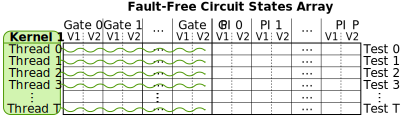
\includegraphics[width=\linewidth]{fig_gpu_k1}
\caption{Kernel 1 uses one GPU thread per two-vector test, with each thread performing a complete circuit simulation of all gates in the presence of the specific test.}
\label{fig:trax_gpu_k1}
\end{figure}
%\vskip 0.5em%

\subsubsection{Kernel function: {\tt cudaFaultSimCore()}}
\label{sec:trax_gpu_cuda_fault_sim_core}
This function is the core of the GPU fault simulator, and is called from both Kernel 1 (fault-free circuit simulation) and Kernel 3 (faulty circuit simulation).
%
The function is called once for each gate evaluation, and is described by the pseudocode in Algorithm~\ref{alg:trax_gpu_cudaFaultSimCore}.

\begin{algorithm}
\centering
\caption[GPU Kernel Function: \texttt{cudaFaultSimCore(gate, myState)}]{-- Kernel Function: \texttt{cudaFaultSimCore(gate, myState)}}
\label{alg:trax_gpu_cudaFaultSimCore}
\begin{algorithmic}[1]
\STATE in1v1 = myState[gate.in1 $\times$ 2]
\STATE in2v1 = myState[gate.in2 $\times$ 2]
\STATE in1v2 = myState[gate.in1 $\times$ 2 + 1]
\STATE in2v2 = myState[gate.in2 $\times$ 2 + 1]
\STATE v1 = gateEval(gate.type, in1v1, in2v1)
\STATE v2 = gateEval(gate.type, in1v2, in2v2)
\IF{hazardProduced(gate.type, in1v1, in1v2, in2v1, in2v2)}
  \STATE v2 = H
\ENDIF
\STATE myState[gate.id $\times$ 2] = v1
\STATE myState[gate.id $\times$ 2 + 1] = v2
\end{algorithmic}
\end{algorithm}

In \verb+cudaFaultSimCore()+, the input values to the current gate are loaded from the \verb+myState+ array in lines 1-4, and are used to compute the gate outputs to vector 1 and vector 2 (\verb+v1+ and \verb+v2+, respectively, in lines 5 and 6) using the gate evaluation lookup table.
%
The four input values are then used in line 7 to determine if a hazard is produced at the output of this gate, and if so, the value of \verb+v2+ is set equal to \textit{H} (line 8).
%
Finally, the \verb+myState+ array is updated with the computed gate-output values \verb+v1+ and \verb+v2+ in lines 10 and 11.

\subsubsection{Kernel 2 - Fault Activation Detection}
\label{sec:trax_gpu_k2}

In general, each two-vector test will activate only a subset of faults in the circuit, and the total fault simulation runtime can be reduced by simulating only the activated faults.
%
Although a TRAX fault, in theory, can also be activated by noise, we only consider here the following two situations:
\begin{enumerate}
\item A conventional gate output transition, either rising or falling.
%
An individual TRAX fault is either a ``slow to rise'' (STR) or a ``slow to fall'' (STF) fault, and in this activation situation, can only be activated by the corresponding gate output transition.
%
\item A hazard is present at the gate output, due to either hazard-causing inputs to the gate, or due to a hazard input value propagating through the gate.
%
There is no differentiating STR versus STF in this case since a hazard implies both a potential rising and falling transition.
\end{enumerate}

Each gate has two potential TRAX faults (a STR and STF fault), as shown in Figure~\ref{fig:trax_gpu_k2}.
%
The GPU fault simulator considers each fault independently, including the two faults belonging to a particular gate, using a separate thread for each fault.
%
Even in the situation where there is a hazard value at a gate output, which would activate both the STR as well as the STF fault, each GPU thread in Kernel 2 only considers a single fault.

Kernel 2 analyzes the fault-free circuit states array (generated by Kernel 1) to determine which faults are activated by which tests, and therefore need to be fault simulated to determine the output errors generated by the activated fault, if any.
%
Before launching the GPU kernel, the GPU memory is allocated to store a one-bit flag for each fault/test, indicating whether or not the fault is activated by the test (with a default value of ``not activated'').
%
Kernel 2 allocates one thread per fault, and each thread checks all tests to determine which tests activate its corresponding fault.

\begin{algorithm}
\centering
\caption[GPU Kernel 2: Fault Activation Detection]{-- Kernel 2: Fault Activation Detection}
\label{alg:trax_gpu_k2}
\begin{algorithmic}[1]
\STATE faultID = (blockID $\times$ BLOCKSIZE) + threadID
\IF{faultID $<$ numFaults}
  \STATE gateID = faultID / 2
  \COMMENT{two faults per gate}
  \STATE risingFault = faultID \% 2
  \COMMENT{even = STF, odd = STR}
  \FOR{testID = 0 \TO (numTests - 1)}
    \STATE myState = allStates + (bytesPerState $\times$ testID)
    \STATE v1 = myState[gateID $\times$ 2]
    \STATE v2 = myState[gateID $\times$ 2 + 1]
    \IF{(risingFault \AND (v1 =\,= 0) \AND (v2 =\,= 1)) \OR\\(\NOT risingFault \AND (v1 =\,= 1) \AND (v2 =\,= 0)) \OR\\(v2 =\,= H) )}
      \STATE markActivated(faultID, testID)
    \ENDIF
  \ENDFOR
\ENDIF
\end{algorithmic}
\end{algorithm}

Kernel 2 is described by the pseudocode in Algorithm~\ref{alg:trax_gpu_k2}.
%
Each thread of Kernel 2 first computes its \verb+faultID+ value (line 1) and only continues execution if it is less than the total number of faults (line 2).
%
The kernel computes the corresponding \verb+gateID+ (line 3) and determines in line 4 if its fault is an STR or STF fault (STF faults have an even \verb+faultID+ while STR faults have an odd \verb+faultID+).
%
Each GPU thread iterates over all tests (lines 5-12) and analyzes the \verb+v1+ and \verb+v2+ values at the fault site (lines 7-8).
%
The first two clauses of the if-conditional in line 9 check for the conventional activation involving a rising or falling transition affecting an STR or STF fault, respectively.
%
The final clause checks for the unique TRAX activation condition, where there is a hazard at the gate output.
%
If any of these conditions occur, the thread marks this fault as activated by this test in line 10.
%
A graphical representation of Kernel 2 is shown in Figure~\ref{fig:trax_gpu_k2}.

%\vskip 0.5em%
\begin{figure}[hbtp]
\centering
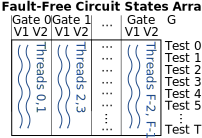
\includegraphics[width=0.5\columnwidth]{fig_gpu_k2}
\caption{Kernel 2 allocates two GPU threads per gate (one each for the STR and STF faults of the gate), where each thread analyzes the data for one gate in the fault-free circuit states array from Kernel 1 to determine which tests cause fault activation.}
\label{fig:trax_gpu_k2}
\end{figure}
%\vskip 0.5em%

After Kernel 2 has finished, the resulting fault activation information is transferred to the CPU for further processing, specifically to create three condensed arrays of fault activation data, as shown in Figure~\ref{fig:trax_gpu_activations_output}.
%
For each fault, in order, the activating \verb+testID+ values are all stored into the activating test IDs array.
%
Second, the total number of activations for each fault is recorded into the second array.
%
Finally, the fault activation counts are used to compute ``fault activation offsets'' for the faults, which determines the starting position of the \verb+testID+ values for the fault in the activating \verb+testIDs+ array.
%
These three arrays are used by the threads of Kernel 3 to identify which tests must be fault simulated.

%\vskip 0.5em%
\begin{figure}[hbtp]
\centering
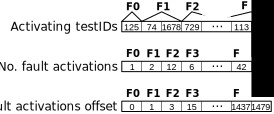
\includegraphics[width=0.8\columnwidth]{fig_gpu_activations_output}
\caption{The fault activation information generated by Kernel 2 is post-processed into the three arrays illustrated here, each of which is used by the threads of Kernel 3.}
\label{fig:trax_gpu_activations_output}
\end{figure}
%\vskip 0.5em%

\subsubsection{Kernel 3 - Fault-Effect Propagation}
\label{sec:trax_gpu_k3}

The final step of the fault simulation process is to determine how each activated fault affects the circuit primary outputs, with the end goal of finding which faults are detected by which tests.
%
Naturally, faults that are not activated by a given test will not be detected, so the fault simulator only performs fault simulation for activated faults for the tests that activate them, significantly reducing the required computation time.

In general, fault simulation is very similar to the fault-free circuit simulation of Kernel 1, which is the reason that the \verb+cudaFaultSimCore()+ function was created, enabling it to be used for both purposes.
%
However, there is one crucial difference here, in that the activated fault site must be identified as producing the output value \textit{X} (according to the TRAX fault model).
%
After this activation, fault simulation continues as in Kernel 1, as a gate-by-gate re-evaluation of the circuit.

Additionally, an optimization called ``skip ahead'' is used here to accelerate the parallel fault simulation.
%
Given that the circuit netlist gates are stored in topological order, an activated fault at gate $n$ cannot affect any gates that come before it, meaning that gate re-evaluation can simply start at gate $n+1$ and proceed to simulate the remaining gates in order.
%
While this optimization results in minimal time reduction for faults occurring early in the topological order, a significant amount of time reduction is observed for gates occurring later in the order.

Due to the fact that the concurrent simulation of different faults would require each thread to start at a different location in the gate ordering (unlike in Kernel 1, where all faults start at \verb+gateID=0+ and proceed in lock-step), Kernel 3 is designed to simulate the activations and fault-effect (i.e., \textit{X} value) propagations of a single fault for all activating two-vector tests, requiring one invocation of Kernel 3 for each fault in the circuit.
%
While this incurs a small amount of overhead for each kernel invocation, there are significant advantages to this approach, including enabling the skip-ahead optimization, avoiding branch-divergence between threads simulating different fault sites, and, especially, limiting the amount of memory required for Kernel 3.
%
The pseudocode of Kernel 3 is shown in Algorithm~\ref{alg:trax_gpu_k3}, and a graphical representation is given in Figure~\ref{fig:trax_gpu_k3}.

\begin{algorithm}
\centering
\caption[GPU Kernel 3: Fault-Effect Propagation]{-- Kernel 3: Fault-Effect Propagation}
\label{alg:trax_gpu_k3}
\begin{algorithmic}[1]
\STATE testOffset = (blockID $\times$ BLOCKSIZE) + threadID
\STATE faultOffset = faultActivationsOffset[faultID]
\IF{testOffset $<$ numFaultActivations[faultID]}
  \STATE testID = activatingTestIDs[faultOffset + testOffset]
  \STATE myState = allStates + (bytesPerState $\times$ testID)
  \STATE myGateID = faultID / 2
  \COMMENT{two faults per gate}
  \STATE myState[myGateID $\times$ 2 + 1] = X
  \COMMENT{activate the fault}

  \COMMENT{Simulation starts with the next gate}
  \FOR{gateID = (myGateID + 1) \TO (numGates - 1)}
    \STATE gate = gates[gateID]
    \STATE cudaFaultSimCore(gate, myState)
    \IF{gate.isOutput \AND myState[gateID $\times$ 2 + 1] =\,= X}
      \STATE markFaultDetected(faultID, testID)
    \ENDIF
  \ENDFOR
\ENDIF
\end{algorithmic}
\end{algorithm}

%\vskip 0.5em%
\begin{figure}[hbtp]
\centering
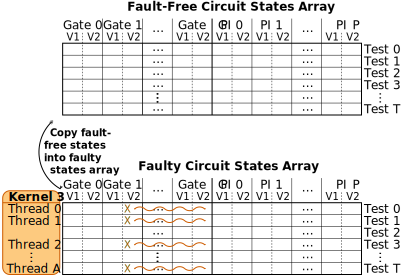
\includegraphics[width=\linewidth]{fig_gpu_k3}
\caption{Kernel 3 is invoked once per fault, and allocates one GPU thread per activated fault, which is designated by injecting an X value at the fault site and then simulating those gates that follow the fault site in the topologically-ordered list.}
\label{fig:trax_gpu_k3}
\end{figure}
%\vskip 0.5em%

Under this scheme, the GPU maintains in memory the fault-free circuit states from Kernel 1 (one state for each two-vector test).
%
For each invocation of Kernel 3 (for each fault to be simulated), the GPU makes a device-to-device memory copy of the fault-free circuit states to a temporary ``faulty circuit states'' memory location.
%
This is a constant amount of memory and does not depend on or scale with the number of activating tests for a given fault.

Each thread of Kernel 3 first computes its \verb+testOffset+ and \verb+faultOffset+ (lines 1-2) and only continues execution if the test offset is less than the total number of activations for this fault (line 3).
%
Kernel 3 uses the arrays shown in Figure~\ref{fig:trax_gpu_activations_output} to determine the corresponding \verb+testID+ (line 4), which serves as an index into the faulty circuit states array.
%
The gate corresponding to the current fault is determined (line 6), and the fault is activated by injecting an \textit{X} value at the fault site (line 7).
%
As part of the skip-ahead optimization, the gate loop in line 8 starts with \verb+gateID+ equal to the next gate after the fault site gate, simulating (line 10) each remaining gate in turn.
%
If a gate drives a circuit primary output and has an \textit{X} value as output (line 11), the fault has been detected, and the kernel records this in the fault dictionary data structure in line 12.

Given that the final output of the fault simulation (the pass/fail dictionary data) is a single bit for each fault/test pair, it would be inefficient to copy the complete faulty circuit states array from GPU to CPU after each invocation of Kernel 3, only to have the CPU determine the pass/fail bits from the circuit states, discarding a majority of the transferred data.
%
Instead, the fault dictionary data structure is created in GPU memory before any invocations of Kernel 3, initialized to have no faults marked as detected.
%
As each fault activation is simulated, the fault dictionary data structure in the GPU memory is updated with the fault detection status.
%
After all faults are simulated, the completed fault dictionary is finally transferred from GPU to CPU, where it is then copied to non-volatile memory.

In summary, fault dictionaries are indispensable for performing on-chip diagnosis but require significant computational resources to construct.
%
The inherent parallelism of fault simulation makes it an ideal candidate for acceleration through the use of a GPU.
%
The CUDA-based GPU-accelerated fault simulator for TRAX faults described here is a straightforward and efficient way to perform the necessary fault simulations required to generate a TRAX fault dictionary, and will be shown to be practical in comparison with a commercial fault simulator by experiments in Section~\ref{sec:trax_exp_gpu}.


\section{Experiments}
\label{trax_exp}

Several experiments are performed to evaluate the TRAX fault model and GPU-accelerated fault simulation.
%
A gate-level simulation experiment comparing TF and TRAX fault responses is described in Section~\ref{sec:trax_exp_fault_effects}, and a series of experiments on various benchmark circuits are presented in Section \ref{sec:trax_exp_gpu}.

\subsection{Comparison of TRAX and TF Fault Effects}
\label{sec:trax_exp_fault_effects}

To further explore and validate the TRAX subsumption of TF fault responses, we perform a series of circuit simulation experiments on a number of benchmark and other circuits.
%
Fault simulation is used to determine the number of tests that detect each simulated fault, as well as determine the count of failing circuit outputs.
%
This fault simulation is performed for both TRAX and TF faults, for four different benchmark circuits.
%
The resulting counts of fault detecting tests and failing output bits are normalized for each circuit to permit cross-circuit comparison.

%\vskip 0.2em%
\begin{figure}[hbtp]
\centering
\includegraphics[width=0.9\columnwidth]{fig_norm_output_count}
\caption{Each point above represents a single fault, positioned to indicate the relative count of failing circuit outputs between TRAX and TF fault simulation, for four different benchmark circuits.
%
The results demonstrate that TRAX fault effects subsume TF fault effects.}
\label{fig:norm_output_count}
\end{figure}
%\vskip 0.5em%

%\vskip 0.2em%
\begin{figure}[hbtp]
\centering
\includegraphics[width=0.9\columnwidth]{fig_norm_detection_count}
\caption[Each point above represents a single fault, positioned to indicate the relative count of failing tests between TRAX and TF fault simulation, for four different benchmark circuits.
%
The results demonstrate that TRAX fault detections subsume TF fault detections.]{Each point above represents a single fault, positioned to indicate the relative count of failing tests between TRAX and TF fault simulation, for four different benchmark circuits.
%
The results demonstrate that TRAX fault detections subsume TF fault detections.
%
(Note that it is possible that the corresponding TF and TRAX faults are failing at different outputs even though TRAX has the same or larger count.)}
\label{fig:norm_detection_count}
\end{figure}
%\vskip 0.5em%

Figures~\ref{fig:norm_output_count} and \ref{fig:norm_detection_count} show a scatter plot comparison between TRAX and TF fault responses for each simulated fault.
%
Each point in these two figures is a single simulated fault, where the position is determined by the normalized count of failing outputs (Figure~\ref{fig:norm_output_count}) or detecting tests (Figure~\ref{fig:norm_detection_count}) for TRAX and TF simulations of that fault.
%
A line is drawn to indicate where TRAX and TF have equal counts.
%
We observe that for both detections and failing output count, for every fault, the TRAX behavior subsumes the TF behavior, as made evident by no faults falling below the indicated line.

\subsection{TRAX Fault Simulation Acceleration}
\label{sec:trax_exp_gpu}

A series of experiments evaluate both the accuracy and acceleration of the GPU TRAX fault simulator.
%
Due to the unavailability of a TRAX-compatible commercial fault simulator, a single-threaded CPU reference implementation is used to verify the accuracy of the GPU fault simulator using two-vector tests created by a commercial ATPG tool targeting conventional transition faults.
%
For all circuits and two-vector tests, there are no discrepancies between the reference implementation and the accelerated GPU implementation.

To evaluate runtime performance, the GPU simulator is compared to a commercial fault simulation tool that is used with conventional transition faults.
%
Although the commercial tool is unable to fully implement the features of the TRAX fault model (and instead simulates transition faults), a comparison of the two execution times is worthwhile.
%
As previously mentioned, each large gate has been replaced by an equivalent subcircuit of two-input gates to simplify the GPU fault simulation.
%
The set of faults to simulate is generated from the original netlist (before large gates are replaced), and this fault set is provided to both the commercial tool and the GPU fault simulator to ensure a fair comparison.
%
Because the two-vector test set is generated as part of the commercial tool ATPG process, the tool writes the test set to disk so it can be imported into the GPU fault simulator, ensuring that the same tests are used for both fault simulation tools.
%
The commercial fault simulation tool is running on a 2.2 GHz Xeon E5-4620 (single-threaded fault simulation), and the GPU fault simulation is running on a Nvidia GTX-1080 GPU.

%\vskip 0.5em%
\begin{table}[hbtp]
\centering
\begin{tabular*}{1.0\columnwidth}{@{\extracolsep{\fill}}|l|rr|r|rr|}
\hline
                                &\multicolumn{2}{c|}{GPU (s)}       &\multicolumn{1}{c|}{CPU (s)}   &\multicolumn{2}{c|}{Speedup}\\
\hline
Circuit (No. gates, No. tests)  &TRAX       &TF                     &TF                             &TRAX   &TF\\
\hline
c432 (208, 37)                  &0.148      &0.123                  &1.895                          &12.76  &15.37\\
c499 (246, 71)                  &0.130      &0.124                  &2.469                          &19.00  &19.88\\
c1355 (558, 106)                &0.281      &0.243                  &4.809                          &17.11  &19.79\\
c1908 (368, 64)                 &0.154      &0.144                  &2.376                          &15.45  &16.48\\
c2670 (1,168, 67)               &0.658      &0.539                  &8.779                          &13.35  &16.30\\
c3540 (1,512, 128)              &1.181      &0.942                  &12.346                         &10.46  &13.11\\
c5315 (2,740, 85)               &3.177      &2.444                  &23.691                         &7.46   &9.69\\
c7552 (3,223, 84)               &4.750      &3.582                  &29.963                         &6.31   &8.36\\
\hline
b12 (1,336, 80)                 &0.641      &0.506                  &7.375                          &11.50  &14.58\\
b14\_opt (6,878, 345)           &39.377     &23.439                 &201.311                        &5.11   &8.59\\
b14 (10,682, 657)               &201.269    &77.986                 &1,009.105                      &5.01   &12.94\\
b15 (9,877, 407)                &81.045     &46.432                 &503.040                        &6.21   &10.83\\
b17\_opt (30,396, 600)          &907.294    &453.962                &4,996.472                      &5.51   &11.01\\
b18\_opt (90,729, 704)          &9,015.342  &4,551.655              &51,812.517                     &5.75   &11.38\\
b22 (32,247, 554)               &1,676.197  &558.607                &5,303.097                      &3.16   &9.49\\
\hline
L2B (12,222, 90)                &83.655     &58.413                 &550.146                        &6.58   &9.42\\
NCU (78,677, 211)               &1,755.930  &1,243.913              &15,033.808                     &8.56   &12.09\\
\hline
epflDiv (101,603, 612)          &17,198.853 &8,390.128              &50,236.483                     &2.92   &5.99\\
epflMult (50,504, 77)           &1,338.662  &1,026.140              &2,668.724                      &1.99   &2.60\\
epflSqrt (41,042, 161)          &1,185.846  &810.855                &2,945.845                      &2.48   &3.63\\
epflSquare (35,492, 79)         &661.580    &527.172                &1,404.470                      &2.12   &2.66\\
epflMemCtrl (82,538, 1,276)     &13,870.393 &8,427.150              &93,803.048                     &6.76   &11.13\\
\hline
\multicolumn{4}{|r|}{Average:}                                                                      &7.98   &11.15\\
\multicolumn{4}{|r|}{Maximum:}                                                                      &19.00  &19.88\\
\hline
\end{tabular*}
\caption{Fault simulation (with no fault dropping) is performed using the GPU fault simulator (for TRAX and TF models) as well as a commercial fault simulator (TF model only) in order to compare the runtime of each.
%
The speedup results compare the GPU TRAX and TF runtimes with the CPU (commercial tool) TF runtimes.}
\label{table:trax_exp_gpu_runtime_comparison}
\end{table}
%\vskip 0.5em%

Comparative fault simulation results (without fault dropping) are shown in Table~\ref{table:trax_exp_gpu_runtime_comparison}.
%
The GPU fault simulator can perform both TF and TRAX fault simulation, while the commercial tool can only perform TF fault simulation.
%
The GPU and commercial-tool runtimes are reported in seconds, and the speedup comparisons are shown in the final two columns.
%
The highest speedup is achieved for the smaller ISCAS85~\cite{brglez85} benchmark circuits, with a declining speedup as circuit size increases.
%
The EPFL circuits~\cite{epfl}, in addition to being some of the largest circuits analyzed, generally show the least speedup.
%
Overall, when comparing the TF runtimes between the GPU and CPU implementations, the average speedup is 11.15x with a maximum speedup of 19.88x.
%
Due to the increased number of fault activations when performing TRAX fault simulation as compared to TF fault simulation, the TRAX fault simulations achieved less of a speedup than for TF.
%
For TRAX the average speedup achieved is 7.98x, with a maximum speedup of 19x.
%
When comparing GPU fault simulation runtimes for the TF and TRAX fault models, we observed that GPU TF fault simulation was 1.5x faster than TRAX fault simulation, on average.
%



\section{Summary}
\label{sec:trax_summary}

Targeting the gradual slowdowns of early-life and wear-out failures, the TRAX fault model is a new enhancement to the unspecified-transition fault model~\cite{pomeranz08}.
%
TRAX faults conservatively and efficiently capture all possible activation and propagation paths for a speed-degraded standard cell.
%
Whether activated by a conventional gate output transition or activated by a hazard, a TRAX fault generates an \textit{X} value that encompasses all possible transport delays through that gate.
%
Designed to subsume all potential delay fault effects, fault simulation has shown that the TRAX model does indeed subsume the fault effects of the TF model.
%
To counter the large amount of computation required to generate the fault dictionary, a GPU-accelerated fault simulation engine has been developed.
%
Fault simulation experiments show an average speed-up of nearly 8x for the GPU fault simulator when compared to a leading commercial tool.


\chapter{Hierarchical Fault Dictionary}
\label{chap:dict}

The goal of on-chip test and diagnosis is to provide robustness against early-life and wear-out failures, through periodic self-test and self-diagnosis.
%
Once a test failure is detected, the failure must be localized (diagnosed) to determine which module of the tested core/uncore is defective.
%
A fault dictionary is one method of performing fault diagnosis, and the dictionary is a pre-computed table of expected circuit behavior in the presence of each modeled fault.
%
For testing a complex modern System on Chip (SoC), a high-quality set of two-vector tests plus a fault dictionary are created for each unique core or uncore in the SoC.
%
During normal operation in the field, the test and diagnosis controller selects a core/uncore for test, isolates it from the rest of the SoC, applies the corresponding test set while recording the test responses, and upon detecting failure, finally uses the fault dictionary and the recorded test responses for localization via the on-chip diagnosis hardware.

As previously mentioned, the few economically-feasible recovery options available at runtime (namely to repair, replace, or avoid a defect) are too expensive to be implemented at a fine level of granularity.
%
That is, it is not viable to repair a single transistor, or replace a particular flip-flop.
%
These recovery actions are only practical for larger modules at a higher level of the design hierarchy.
%
While the goal of conventional fault diagnosis is to localize the failure to a specific modeled fault, on-chip diagnosis only needs to localize a failure to the level of repair, replacement, or avoidance, also known as the level of \textit{recovery}.
%
This relaxation of diagnosis precision enables the removal of faults from the dictionary that are not necessary for performing recovery-level diagnosis.

A fault dictionary is a tabulation of expected circuit responses (or some subset thereof) for each modeled fault considered, for each test (or test pair) in the test set.
%
It is convenient to view a fault dictionary as a table of values (fault simulation responses) with one row for each fault and one column for each test pair.
%
A fault dictionary that contains the full response for each fault/test pair is a \textit{full-response dictionary}.
%
Traditional diagnosis searches the rows of the fault dictionary to find the fault that matches (or is the most similar to) the observed behavior of a faulty circuit.
%
For the TRAX fault model, where an exact match between a modeled fault and defective circuit is not expected, a more complex diagnosis process is required, as detailed in Chapter~\ref{chap:diag}.
%
The rest of this chapter details the creation of a new fault dictionary with increased compaction, owing to the reduced recovery-level localization requirements of on-chip diagnosis.

A full-response fault dictionary requires a large amount of storage, equal to the product of the number of faults, the number of tests, and the number of circuit primary outputs, which can be quite large for modern designs.
%
For example, the circuit L2B~\cite{sun11} contains just over 12,000 gates and uses 90 test vector pairs for test and diagnosis.
%
The full-response fault dictionary for L2B requires over 600 megabytes of storage, which is impractical for on-chip diagnosis for this relatively small circuit.
%
To reduce the size required to store a fault dictionary, a variety of compaction schemes~\cite{arslan02, bernardi06, boppana94, chakravarty99, boppana96, chess99, hong07, pomeranz92} have been developed for reducing the size of a fault dictionary, each exhibiting their own trade-off between diagnostic resolution and dictionary size/complexity.
%
Existing techniques are effective but do not enable a sufficient level of compaction when applied to modern designs~\cite{ryan93, boppana94}.
%
One straightforward compaction technique is only to include faults relating to the targeted defect model (i.e., NBTI and ELF).
%
To this end, the TRAX fault dictionary explored here only includes faults located at standard-cell outputs since NBTI and ELF affect the delay of standard cells.
%
Elimination of the remaining faults (i.e., faults located at primary inputs or fanout branches) reduces dictionary size through the removal of dictionary rows.

Given that system resources for test and diagnosis must be limited, it is not feasible to store the entire simulation response of every fault.
%
Instead, a single bit per test is stored to indicate pass/fail status of the corresponding simulation response, resulting in a pass/fail dictionary.
%
A pass/fail dictionary is a well-known technique for significantly reducing the size of a fault dictionary at the expense of diagnostic resolution~\cite{pomeranz92}.
%
Resolution degradation, however, is minimal since the level of precision required is limited to the level of recovery.
%
Specifically, for all benchmark circuits analyzed, the resolution loss averaged less than 0.023\%, where resolution is equated to the number of distinguished fault pairs divided by the total number of fault pairs.

\section{Module-Level Hierarchy}
\label{sec:dict_mod_level_hier}

For on-chip test and diagnosis, the tested core or uncore~\cite{li08, inoue08} is assumed to be partitioned into a set of interconnected modules, each of which can be independently repaired, replaced, or avoided if found to be faulty.
%
Figure~\ref{fig:dict_core_uncore_modules_faults} illustrates an example system-on-chip (SoC) that contains three cores/uncores which themselves are composed of multiple modules that include TRAX faults shown as circles within each module.
%
The modules within each core/uncore are assumed to be at the recovery-level.
%
In other words, these modules are at the finest level of granularity for which recovery can be cost-effectively deployed.
%
Put another way, it would be ideal if the actual transistor responsible for slowdown could be both identified and handled via repair, replacement, or avoidance.
%
Achieving robustness however at this very fine level of granularity is much too costly.
%
So instead, the level of recovery is defined to be the set of sub-circuits (i.e., modules) within a core or uncore that can be effectively handled by repair, replacement, or avoidance.
%
We make no assumptions however how small or large these modules should be since there are challenging tradeoffs involving performance, power, and robustness.
%
Regardless of how these modules are defined, the approach for on-chip diagnosis described here remains applicable, albeit with an associated level of efficiency and effectiveness that is dependent on core/uncore partitioning into modules.
%
Finally, it is also important to point out that the core/uncore is the smallest testable entity.
%
That is, we assume it is not cost-effective to test each module within a core/uncore separately from all other modules.
%
If this were not true, then diagnosis would be unnecessary since test failure alone would identify the culprit module.

%\vskip 0.5em%
\begin{figure}[hbtp]
\centering
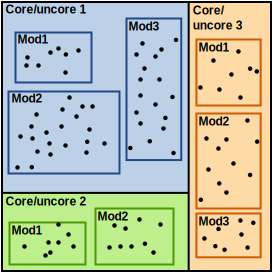
\includegraphics[width=0.4\columnwidth]{fig_core_uncore_modules_faults}
\caption{Hierarchical view of a system-on-chip (SoC) that contains multiple cores and uncores, each of which contain multiple modules.
%
Within each module are a number of faults.}
\label{fig:dict_core_uncore_modules_faults}
\end{figure}
%\vskip 0.5em%

One example of sub-module repair is presented in~\cite{hsiung15}, where a multi-layered approach is used to provide defect-tolerance and improve yield.
%
The layers analyzed include circuit-, microarchitecture-, and ISA-layers.
%
At each layer, workload analysis is used to determine if there are any sub-modules that occupy a disproportional amount of the workload or circuit area, potentially leading to a more fine-grained repair option.
%
As an example, for the ALU analyzed at the microarchitecture-layer, the coarse approach would be to disable an entire ALU found to be faulty.
%
Through workload and circuit analysis, the multiplier sub-module is determined to occupy a large percentage of the ALU area, and that a majority of multiplication operations performed only require accuracy in the lower $N$ bits of the product.
%
This permits a more fine-grained repair approach where such limited-output-size multiply operands can continue to use such a partially-damaged ALU.
%
As another example, many circuits contain arrays of identical structure, such as the full-adder blocks of a multi-bit adder module.
%
The approach presened in~\cite{hsiung15} recognizes that if the repeated circuit structures are not all free from defects, a small amount of additional data steering logic can be used to iteratively perform a calculation with partially-faulty hardware.
%
While this paper does not address the diagnosis process necessary to determine which module or sub-modules are faulty, it does provide an example of circuit repair performed within a single block of combinational logic, much like the approach assumed in this dissertation.

Because of the recovery level, on-chip diagnosis is significantly eased as compared to conventional approaches since precision can be relaxed to the module-level of localization.
%
Existing dictionary compaction techniques have not considered this relaxation in diagnosis precision and are therefore not directly applicable to the on-chip diagnosis task formulated here.
%
In other words, diagnosing to the recovery level means that circuit-level resolution (e.g., signal line, standard cell, or layout) can be replaced with module-level resolution to achieve a smaller dictionary size.
%
In addition, this means that only certain inter-module fault pairs have to be distinguished within the fault dictionary (i.e., have dictionary rows where at least one entry is different).


\section{Fault Equivalence and Subsumption}
\label{sec:dict_fault_equ_sub}

For intra-module faults that are test-set equivalent (identical simulation responses for all tests), all but one can be eliminated since distinguishing them using advanced diagnosis techniques (e.g.,~\cite{desineni05}) is now unnecessary.
%
Other intra-module faults can also be eliminated based on subsumption.
%
Subsumption is similar to dominance but is subtly different due to the use of the \textit{X} value and the opposite way it is exploited to reduce the fault universe.
%
A fault $c$ is said to subsume another fault $d$, if $c$ and $d$ are not test-set equivalent and the erroneous test response of $c$ subsumes the erroneous response of $d$.
%
In other words, fault $c$ subsumes fault $d$ if $c$ produces an \textit{X} value for all the same tests and outputs as fault $d$, and their fault-simulation responses are not identical.
%
A subsumed fault (e.g., fault $d$) can be eliminated since, if it exists, it will produce a response that can also be produced by fault $c$\footnote{It should be noted that fault subsumption is only valid for a fault model such as TRAX since conventional fault models have only a single simulation response.
%
TRAX faults, on the other hand, have a set of possible responses given that the observed X values all do not have to correspond to errors.}.
%
Again, since faults $c$ and $d$ are in the same module, there is no need to distinguish them.
%
Note that the subsuming fault (e.g., fault $c$) cannot be eliminated since it could produce a response that is not captured by another fault in the module, thus making it possible that it would not be distinguished from some other fault outside the module if it were removed.

Using subsumption to eliminate faults is not the same as dominance-based fault collapsing.
%
First, in dominance collapsing, the dominating fault (e.g., fault $c$) is the one collapsed.
%
Second, and more importantly, dominance-collapsed faults cannot be altogether eliminated in an application such as ATPG since they must still be explicitly considered if a test cannot be found for any of its dominated faults.

%\vskip 0.5em%
\begin{table}[hbtp]
\centering
\begin{tabular*}{0.9\columnwidth}{@{\extracolsep{\fill}}cccccccl}
\toprule
Fault&Module&$T_1$&$T_2$&$T_3$&$T_4$&$T_5$&\\
\midrule
$F_1$&$M_1$&P&F&F&P&F&\\
$F_2$&$M_1$&P&F&F&P&F&Eliminated (EQU)\\
$F_3$&$M_1$&P&F&P&P&P&Eliminated (SUB)\\
$F_4$&$M_1$&F&F&P&P&F&\\
\midrule
$F_5$&$M_2$&F&F&P&P&F&\\
$F_6$&$M_2$&P&P&F&F&P&\\
\bottomrule
\end{tabular*}
\caption{TRAX fault dictionary data illustrates dictionary compaction, using equivalence and subsumption relationships to eliminate two intra-module faults.
%
Specifically, $F_2$ is eliminated due to equivalence with $F_1$, and $F_3$ is eliminated because it is subsumed by both $F_1$ and $F_4$.}
\label{table:dict_fault_resp}
\end{table}
%\vskip 0.2em%

In the context of on-chip diagnosis, where test and diagnosis resources are limited, it is only feasible to store the test responses as a single pass/fail bit.
%
Instead of analyzing full-responses, fault elimination through equivalence and subsumption is performed using the pass/fail response from each test.
%
An example of this process is shown in Table~\ref{table:dict_fault_resp}.
%
Specifically, fault $F_2$ is eliminated via equivalence with $F_1$, and $F_3$ is eliminated because it is subsumed by both $F_1$ and $F_4$.
%
These two techniques for fault reduction are only applied to faults belonging to the same module because recovery-level diagnosis does not require distinguishing intra-module faults.
%
Applying these dictionary compaction techniques produces a \textit{collapsed pass/fail hierarchical dictionary}, which is used in the diagnosis experiments presented later.
%
For the L2B fault dictionary mentioned before, the full-response dictionary of over 600 megabytes is compacted to less than 32 kilobytes for the collapsed pass/fail dictionary.


\section{Experiments}
\label{sec:dict_exp}
A variety of experiments are performed to evaluate a collapsed pass/fail hierarchical dictionary based on the TRAX fault model.
%
Specifically, hierarchical fault dictionaries are built for 22 benchmark circuits, for the TF, TRAX, and UTF fault models, presented in Section~\ref{sec:dict_exp_size_res}.
%
The sensitivity of diagnosis results to the level of circuit partitioning is analyzed in Section~\ref{sec:dict_exp_partitioning}.


\subsection{Dictionary Size and Resolution}
\label{sec:dict_exp_size_res}

As previously mentioned, measuring dictionary size reduction due to fault elimination requires access to designs that exhibit module-level hierarchy.
%
The hierarchical versions of the ISCAS85 benchmark circuits~\cite{brglez85} (modified by~\cite{hansen99}) serve this purpose since many of the benchmarks have been reverse engineered to at least two levels of hierarchy.
%
Additionally, seven circuits are taken from the ITC99 benchmark set~\cite{corno99}, two circuits are taken from the OpenSPARC T2 design~\cite{sun11}, and five circuits are taken from the EPFL Combinational Benchmarks suite~\cite{epfl}.
%
Unlike the ISCAS85 benchmark circuits, these additional circuits are not pre-partitioned into module-level hierarchy and are instead partitioned into ten modules each using graph clustering software~\cite{dhillon07}.
%
For these experiments, the second-level modules of the circuits are deemed the recovery level.
%
In other words, diagnostic precision must only be achieved at the second level of the hierarchy of these circuits.
%
The generated tests are fault simulated using the TRAX fault model using the GPU-based TRAX fault simulator described in Chapter~\ref{chap:trax}.

%\vskip 0.5em%
\begin{figure}[htbp]
\centering
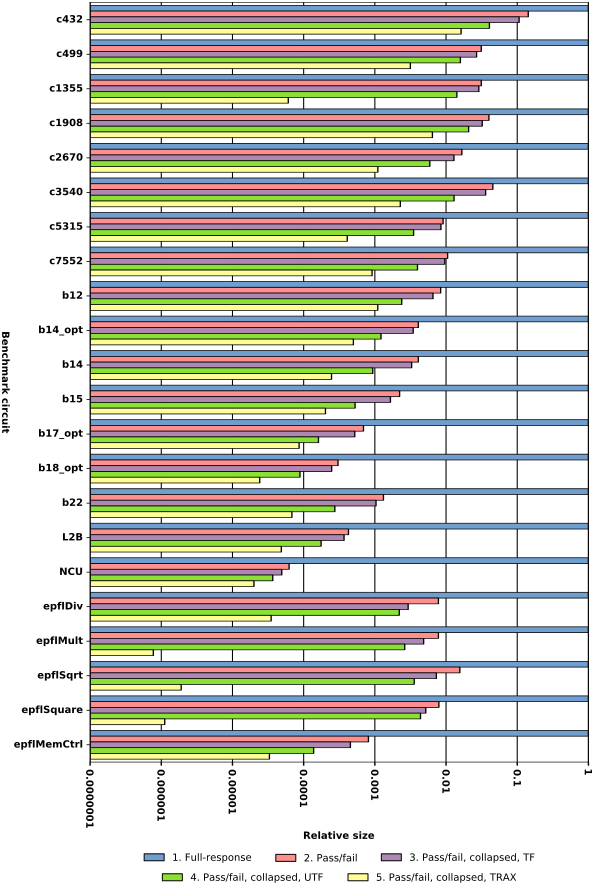
\includegraphics[width=\columnwidth]{fig_dictionary_histogram_vertical}
\caption{Comparison of fault-dictionary size for various compaction techniques.}
\label{fig:dict_histogram}
\end{figure}
%\vskip 0.5em%

Figure~\ref{fig:dict_histogram} shows the amount of dictionary size reduction resulting from the two compaction steps (pass/fail compaction, followed by equivalence and subsumption fault collapsing for the TRAX, UTF, and TF fault models) for several circuits.
%
This results in five fault dictionaries:
\begin{enumerate}
\item Full-response dictionary
\item Pass/fail dictionary
\item Pass/fail, collapsed, TF fault model dictionary
\item Pass/fail, collapsed, UTF fault model dictionary
\item Pass/fail, collapsed, TRAX fault model dictionary
\end{enumerate}
Both equivalence and subsumption fault collapsing are used for the TRAX and UTF dictionaries, however, because subsumption is not valid for the TF model, only equivalence fault collapsing is used for the TF dictionaries, resulting in very little additional compaction for TF.
%
While the use of hazard activation enables the TRAX fault model to subsume any glitch-caused failures in a circuit, the aggressive hazard activations result in the elimination of many faults by subsumption.
%
This produces a much smaller dictionary, but one with reduced diagnostic efficacy (evaluated in Chapter~\ref{chap:diag}).
%
Each design has five bars which show the relative size of each of the five dictionaries, on a logarithmic scale.
%
Each set is normalized to the size of the full-response dictionary.

On average, the dictionary size is reduced by 98.64\% for TF, reduced by 99.37\% for UTF, and reduced by 99.85\% for TRAX.
%
The maximum reduction for a UTF dictionary is for the NCU dictionary, which is compacted down to only 0.003683\% of the original size, a reduction by over 27,000x.
%
This reduces the NCU fault dictionary from 211 GB for the full-response dictionary to under 8 MB for the UTF compacted pass/fail dictionary.
%
For the TRAX dictionaries, the greatest compaction achieved is for the \verb+epflMult+ circuit, compacted down to only 0.00007734\% of the full-response size.
%
However, due to this incredible compaction, the dictionary does not retain much of its diagnostic ability.
%
The high compaction is due to this circuit having a few faults that fail very many of the applied tests.
%
Faults like this will eliminate many of the other faults in the same module via subsumption, leaving few faults (sometimes only one) remaining in each module.
%
Additionally, the EPFL circuits have very few input and output pins given the number of logic gates within each circuit, which reduces both controllability and observability for test generation.
%
Figure~\ref{fig:dict_gates_per_po} shows a plot of the gates per primary output for each analyzed circuit, showing that the EPFL circuits have many more gates per PO than the other benchmark circuits.
%
Further investigation of the often-failing faults is left as an area of future work.

%\vskip 0.5em%
\begin{figure}[htbp]
\centering
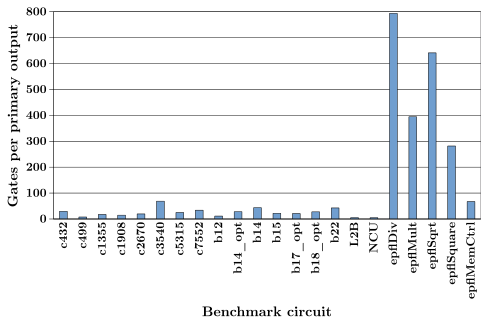
\includegraphics[width=0.8\columnwidth]{fig_dict_gates_per_po}
\caption{Comparison of the number of gates per primary output for each benchmark circuit.}
\label{fig:dict_gates_per_po}
\end{figure}
%\vskip 0.5em%

\subsection{Design Partition Sensitivity}
\label{sec:dict_exp_partitioning}

As previously mentioned, the non-ISCAS85 benchmarks lack any pre-existing module-level hierarchical and are partitioned into ten modules using graph clustering software.
%
A brief analysis is performed to determine the sensitivity of dictionary characteristics to the number of module partitions.
%
This analysis consists of repeatedly performing the following steps:
\begin{enumerate}
\item Use graph clustering to partition the circuit into $m$ modules.
\item Construct and compact the TRAX fault dictionary.
\item Evaluate diagnostic ability of resulting fault dictionary.
\end{enumerate}
These steps are performed for $m$ = 5 to 30, for both the L2B circuit (Figure~\ref{fig:dict_num_modules_clustering_l2b}) and the NCU circuit (Figure~\ref{fig:dict_num_modules_clustering_ncu}).
%
Details of the evaluation of diagnostic ability are provided in Section~\ref{sec:diag_exp_diag}, but in brief, the conventional metrics of Resolution and Accuracy are used here to evaluate a diagnosis result, including the use of \textit{Ideal Accurate} to describe a diagnosis result where the defective module is called-out as the most-likely responsible module.
%
As the number of module partitions increases from 5 to 30, there is a slight downward trend in the percentage of ideal accurate diagnosis results, and an upward trend in the size of the fault dictionary.
%
While it may appear counter-intuitive for the dictionary size to increase as the number of modules increase, which implies fewer faults per module, there is a logical explanation.
%
Dictionary compaction due to equivalence and subsumption is only applied to intra-module fault pairs, so more compaction is possible with larger modules and therefore more intra-module fault pairs.

%\vskip 0.5em%
\begin{figure}[htbp]
\centering
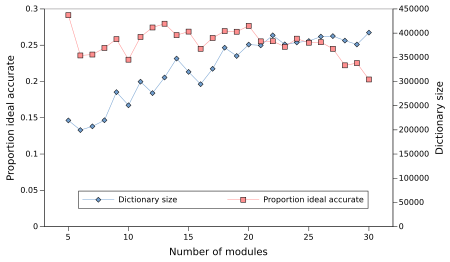
\includegraphics[width=0.9\columnwidth]{fig_dict_num_modules_clustering_l2b}
\caption{Experiments performed for L2B show that as the number of module partitions increase, there is a slight downward trend in ideal accurate diagnoses and a slight upward trend in dictionary size.}
\label{fig:dict_num_modules_clustering_l2b}
\end{figure}
%\vskip 0.5em%

%\vskip 0.5em%
\begin{figure}[htbp]
\centering
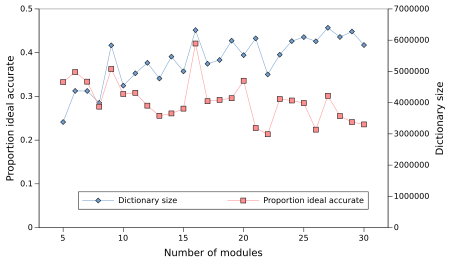
\includegraphics[width=0.9\columnwidth]{fig_dict_num_modules_clustering_ncu}
\caption{Experiments performed for NCU show that as the number of module partitions increase, there is a slight downward trend in ideal accurate diagnoses and a slight upward trend in dictionary size.}
\label{fig:dict_num_modules_clustering_ncu}
\end{figure}
%\vskip 0.5em%

While this may lead to the conclusion that a smaller number of modules is more desirable by these two metrics, this analysis does not include two important considerations.
%
When the number of modules is small, any detected defect will require the repair, replacement, or avoidance of a significant fraction of the core/uncore itself.
%
Furthermore, in the context of replacing modules, this reduces the ability of the core/uncore to recover from any future defects, as more of the available spare modules have been diagnosed as faulty and are unavailable for future use.
%
Taken to extremes, a core/uncore partitioned into a single module would have a zero-byte dictionary with perfect accuracy (every defect is located within the single ``module'' of the core/uncore), but the available recovery options are quite undesirable.
%
It is not very practical to wait to repair an entire core/uncore, replace the entire core/uncore, or try to avoid the core/uncore in its entirety.
%
At the other extreme, a core/uncore partitioned into dozens of modules would have a much larger fault dictionary with an associated reduced percentage of ideal accurate diagnosis results but would have more desirable recovery options available.
%
That is, repairing, replacing, or avoiding a small portion of a defective core/uncore is more appealing than doing the same for the entire core/uncore.
%
Additionally, when considering the replacement of defective modules, smaller and more numerous modules can handle more failures before running out of spare modules.
%
Consider the situation where a single spare is reserved for each module of a core/uncore.
%
If the core/uncore is partitioned into many modules, each can fail independently without reducing the overall functionality of the core/uncore.
%
If there are only a few modules, however, it is more likely that subsequent defects will lie within an already replaced module.

\section{Summary}
\label{sec:dict_summary}

To provide robustness against early-life and wear-out failures, the on-chip test and diagnosis environment localizes any detected failures using a hierarchical fault dictionary.
%
The relaxed diagnosis requirements (requiring defect localization only to the level of recovery) enable significant elimination of dictionary faults determined to be unnecessary for module-level diagnosis.
%
For intra-module faults with equivalent fault responses, all-but-one can be eliminated as redundant.
%
If the fault response of one fault subsumes the fault responses of any other intra-module faults, those subsumed faults can also be eliminated.
%
Dictionary compaction experiments show an average dictionary size reduction by 99.85\% for the TRAX fault dictionary.
%
For one of the largest analyzed circuits (NCU, part of the OpenSPARC T2 processor~\cite{sun11}) the dictionary is compacted down to only 0.00007734\% of the full-response size, reducing the dictionary size from 211 GB down to under 8 MB.
%
Additional analysis to determine the sensitivity of dictionary size and diagnostic ability to circuit partitioning determined a slight positive correlation between the number of partitions and the size of the dictionary, and a slight negative correlation between the number of partitions and the percentage of ideal accurate diagnosis results.
%
This analysis indicates that there is a trade-off to be made between partitioning a core/uncore into a fewer number of modules (with a smaller dictionary size and slightly-improved diagnosis outcome), and a larger number of modules (slightly-larger dictionary size but increased robustness in the face of multiple failing modules).

\chapter{On-Chip Diagnosis Architecture}
\label{chap:diag}

This chapter describes and evaluates a diagnosis architecture developed for performing on-chip diagnosis.
%
While each core/uncore in the System on Chip (SoC) design has a different test set and TRAX fault dictionary, the on-chip diagnosis architecture is used for all diagnosis activities.
%
The CASP test controller~\cite{li08} periodically selects a core/uncore for testing, isolates it from the rest of the SoC (saving critical state and re-routing computational tasks), applies a high-quality test set to the core/uncore while recording the test responses, and finally re-integrates the tested core/uncore within the system (restoring saved state and restoring tasks back to the tested core/uncore).
%
If any failures are detected, the on-chip diagnosis architecture is used to diagnose the failing test responses to localize the failure within the core/uncore.
%
More details on the system test and diagnosis architecture are provided in Section~\ref{sec:diag_system_test_and_diag}.
%
The high-quality test sets needed to detect the targeted early-life and wear-out failures require the use of off-chip storage, which is also used to store the fault dictionary data (details in Section~\ref{sec:diag_off_chip_hw}).
%
The TRAX diagnosis architecture, an on-chip hardware implementation of hierarchical fault diagnosis, is described in Section~\ref{sec:diag_on_chip_hw}.
%
Experiments in Section~\ref{sec:diag_exp} evaluate the on-chip diagnosis architecture.
%
Specifically, we simulate thousands of circuit failures using tests generated by a commercial tool.
%
The ``tester'' response produced by each simulation is fed to the on-chip diagnosis architecture to perform the on-chip diagnosis.
%
The result of each diagnosis is then evaluated for accuracy and resolution, that is, how many faulty modules did diagnosis report (i.e., resolution), and, among the faulty modules reported, did one contain the simulated failure (i.e., accuracy).

\section{System Test and Diagnosis}
\label{sec:diag_system_test_and_diag}

The on-chip test process adopted here leverages CASP (Concurrent Autonomous chip self-test using Stored test Patterns)~\cite{li08}.
%
In CASP, a small amount of additional hardware enables the re-use of DFT logic to test the chip post-manufacturing.
%
High-quality test and diagnosis data are stored in off-chip memory and loaded into the chip as needed during test and diagnosis of a particular core/uncore.
%
Each unique core/uncore in a system requires a set of test and diagnosis data.
%
Off-chip data for each core/uncore is organized as a series of tests, and the data for each test includes (i) a pair of test vector inputs (called $V_1$ and $V_2$), (ii) the expected test response, (iii) a bitmask indicating which response bits should be checked against the expected test response, and (iv) the corresponding column of the fault dictionary.

CASP consists of four phases.
%
First, the CASP controller identifies the next component to test, such as a processing core or an uncore component (e.g., memory controller).
%
Next, the selected core/uncore is then isolated from the rest of the system, saving critical state and re-routing computational tasks.
%
Third, the actual tests are applied one at a time by (i) loading the relevant test data from off-chip into the on-chip buffer, (ii) test application via the DFT logic, and (iii) core/uncore response evaluation for incorrect behavior that results in a one-bit pass/fail status for each test.
%
Finally, once all tests have been applied, the CASP controller reintegrates the core/uncore with the rest of the system and resumes its execution.

The objective of on-chip diagnosis is to determine which module of the core/uncore is most likely the reason for any observed test failure.
%
For on-chip diagnosis, the previously-described TRAX fault dictionary is used, which stores a single bit for fault/test pairs to indicate if the fault is detected by the corresponding test pair.
%
Using the TRAX fault dictionary in conjunction with the pass/fail test response from the CASP test execution, a list of potentially responsible modules is generated.
%
Specifically, starting with a list of all faults within the tested core/uncore dictionary, each failing test response is used one at a time to eliminate any faults that are not detected by the corresponding test.
%
When all test responses have been processed, what remains is a list of TRAX faults consistent with the observed behavior.
%
Each fault in this list belongs to one of the modules of the tested core/uncore.
%
Moreover, counting the number of potentially responsible faults in each module gives an indication of the likelihood of finding the actual defect in each of the implicated modules, and thus is reported as the outcome of on-chip diagnosis.

On-chip diagnosis can be performed in two different situations, the first being failure prediction, where an accelerated clock is used to detect pending failures.
%
In this situation, the diagnosis can be run in the background with no performance overhead and only a little extra power consumption.
%
The other situation is after a real failure is detected, implying that the core/uncore is unable to be used because it has failed.
%
For this case, the time required for diagnosis is indeed important because there is performance overhead associated with diagnosing the failure and deploying fault repair, replacement, or avoidance before execution can resume.


\section{Off-Chip Hardware}
\label{sec:diag_off_chip_hw}

To enable on-chip test and diagnosis requires the addition of specialized hardware, both off and on the chip itself.
%
The off-chip hardware includes memory for storing the test and dictionary data, such as non-volatile flash memory, system DRAM, or on disk.
%
The use of off-chip data storage is reasonable given the trend towards availability of high-density, low-cost flash memory for off-chip storage~\cite{li08}.
%
Additionally, the high-quality test patterns required for ELF and wear-out failure detection cannot easily be produced using conventional BIST techniques.
%
While there are special techniques to achieve high test coverage with BIST~\cite{touba96,wunderlich96}, these techniques can be expensive to implement.
%
Finally, the use of off-chip storage allows the test and dictionary data to be updated (patched), if better-performing data is later identified.
%
Patching might become necessary to deal with a new strain of failure that may occur later in the life cycle of the system, for example, or to incorporate failure knowledge gained from physical failure analysis (PFA) after manufacturing.

%\vskip 0.5em%
\begin{figure}[hbtp]
\centering
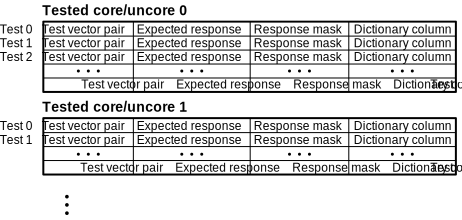
\includegraphics[width=1.0\columnwidth]{fig_off_chip_memory}
\caption{For each unique core/uncore, separate fault dictionaries are constructed and stored in off-chip memory along with the required test data.}
\label{fig:diag_off_chip_memory}
\end{figure}
%\vskip 0.5em%

Each unique core (e.g., CPU, FPU, or GPU) and uncore (DRAM controller, cache controller, etc.) has its own set of test and diagnosis data in the off-chip storage.
%
The use of multiple fault dictionaries, one per tested core/uncore, is justified since it is the smallest testable/repairable object in the chip.
%
Using separate dictionaries reduces the overall amount of dictionary data since faults from the tested core/uncore do not have to be distinguished from all the faults of all the remaining untested cores/uncores.
%
The actual data stored in the off-chip memory is illustrated in Figure~\ref{fig:diag_off_chip_memory}, and consists of an array of test and diagnosis data for each core/uncore, with one row for each test.
%
Additionally, a small amount of core/uncore-specific parameters are stored off-chip, including the fault count, test vector count, and the boundary values used by the diagnosis architecture (Section~\ref{sec:diag_on_chip_hw}) to determine which modeled faults belong to which module of the core/uncore.

The test and diagnosis data stored for each test consists of the pair of test vectors called $V_1$ and $V_2$, which are applied to the core/uncore using (mostly) existing DFT under the control of the CASP test controller~\cite{li08,li10,li13}.
%
Also stored is the expected response of the core/uncore to the applied test vector pair and a response mask indicating the validity of each response bit.
%
Finally, each test also has associated diagnosis data, specifically the corresponding test column of the core/uncore fault dictionary.
%
As previously mentioned, a fault dictionary can be thought of a table of fault responses (or some subset or function of the fault responses) with one row for each modeled fault and one column for each applied test.
%
For a TRAX hierarchical fault dictionary, each column indicates which modeled faults could cause a failure for the corresponding test.
%
A dictionary test column is used for the on-chip diagnosis; specifically, it is used to eliminate faults that could not possibly explain the observed test failures, leaving only those ``candidate'' faults that could be responsible for the faulty behavior.

Details of the size of the off-chip storage deserve further discussion.
%
The test vectors $V_1$ and $V_2$, the expected response, and the response mask all require as many bits as the length of the scan chain for the corresponding core/uncore.
%
The dictionary test column data requires one bit per fault.
%
All of this data (vectors, response, mask, and dictionary column) is repeated for each test in the core/uncore test set.
%
We calculate the required off-chip storage for one of the largest analyzed circuits, the NCU uncore from the OpenSPARC T2 processor design~\cite{sun11}.
%
With 16,582 bits in the scan chain and 21,537 faults in the dictionary, 10.73 KB of off-chip storage are required for each of the 211 tests required for NCU, bringing the total to 2.21 MB.

Because these tests are applied during the normal operation of the system, user-visible test execution time should be minimized.
%
Fortunately, the off-chip test data can be pre-fetched into on-chip buffers during normal operation (before the selected core/uncore is isolated from the system for test), hiding the access and transfer time.
%
If test results indicate that the core/uncore has failed any applied tests, dictionary data is loaded from off-chip storage and used by the diagnosis architecture.
%
When a faulty core/uncore is detected, the system must take some corrective action (repair, replace, or avoid the faulty module), so the additional time required to load the dictionary data is small compared to the recovery time.


\section{TRAX On-Chip Hardware}
\label{sec:diag_on_chip_hw}

In addition to the off-chip storage, there is dedicated on-chip hardware for actually performing diagnosis that we call the Diagnosis Architecture (DA); its structure and operation are given in Figure~\ref{fig:diag_trax_architecture} and Algorithm~\ref{alg:diag_on_chip_diag}, respectively.

\begin{algorithm}
\centering
\caption[On-Chip Diagnosis]{-- On-Chip Diagnosis}
\label{alg:diag_on_chip_diag}
\begin{algorithmic}[1]
\STATE perform test and store response in PF
\STATE reset FI counter and $M$ module counters in FMIC
\STATE initialize $(M - 1)$ module index registers (MIRs)
\FOR{$c = 0$ \TO $\lceil F / k \rceil$}
  \STATE reset fault accumulator (FA[0:$k$-1] = 0)
    \FOR{$i=0$ \TO $(T-1)$}
        \STATE FA[0:$k$-1] $|=$ ({\raise.17ex\hbox{$\scriptstyle\sim$}}fault[$ck$:($c$+1)$k$-1][$i$] \& PF[0])
        \STATE PF = PF $>>$ 1
    \ENDFOR
    \FOR{$i=0$ \TO $(k-1)$}
        \FOR{$j=0$ \TO $(M-1)$}
            \IF{FA[0] == 0}
                \IF{lower\_bound[$j$] $\leq$ FI $<$ upper\_bound[$j$]}
                    \STATE module\_count[$j$]++
                \ENDIF
            \ENDIF
        \ENDFOR
        \STATE FA = FA $>>$ 1
        \STATE FI++
    \ENDFOR
    \FOR{$i=0$ \TO $(T_{max} - T)$}
        \STATE PF = PF $>>$ 1
    \ENDFOR
\ENDFOR
\end{algorithmic}
\end{algorithm}

%\vskip 0.5em%
\begin{figure}[hbtp]
\centering
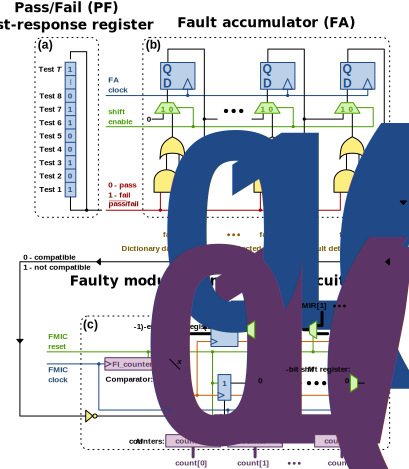
\includegraphics[width=\columnwidth]{fig_trax_architecture}
\caption{The diagnosis architecture: (a) the Pass/Fail (PF) test response register stores test responses in a circular buffer, (b) the fault accumulator (FA) tracks faults compatible with observed incorrect behavior, (c) the faulty module identification circuitry (FMIC) maps faults to core/uncore modules, tracking how many compatible faults are within each module.}
\label{fig:diag_trax_architecture}
\end{figure}
%\vskip 0.5em%

Test execution produces a pass/fail bit for each test vector pair, which is stored in an on-chip circular shift register called the PF (line 1 of Algorithm~\ref{alg:diag_on_chip_diag}, Figure~\ref{fig:diag_trax_architecture}a), where a one indicates the test has failed (Tester Fail) and a zero indicates a test has passed (Tester Pass).
%
The dictionary diagnosis data for the $F$ faults of the tested core/uncore is associated with each test and includes a pass/fail list of $F$ binary values, one per fault, where a one indicates that the corresponding fault is detected by the test (Simulation Fail), and a zero indicates a non-detection (Simulation Pass).
%
The pass/fail test response in the PF is compared with the pass/fail simulation response of each fault (line 7 of Algorithm~\ref{alg:diag_on_chip_diag}).
%
A fault is eliminated if there is any one-sided failure disagreement between the test response and the fault response stored in the dictionary.
%
Specifically, if there is a Tester-Fail Simulation-Pass (TFSP) found for any test, then the corresponding fault is eliminated from consideration.
%
Elimination of a fault using TFSP is justifiable since the TRAX fault model is very conservative in nature.
%
In other words, it is very unlikely for a slowed standard cell to fail a given test without the corresponding fault also being detected given both the generalized activation and fault effect propagation properties that characterize the TRAX fault model (as detailed in Chapter~\ref{chap:trax}, Section~\ref{sec:trax_trax}).

Figure~\ref{fig:diag_trax_architecture}b shows the part of the DA responsible for finding any cases of TFSP.
%
Because the number of faults $F$ for a tested core/uncore can be large, the DA only compares $k < F$ faults at a time, tracked by the variable $c$ in the outer loop (lines 4-24 of Algorithm~\ref{alg:diag_on_chip_diag}).
%
Specifically, for a given test-vector pair $t_i \in T$, its pass/fail response bit stored in the PF is simultaneously compared with the pass/fail simulation bits from $k$ faults (line 7 of Algorithm~\ref{alg:diag_on_chip_diag}).
%
The result of each comparison is stored in a flip-flop; a zero is stored for a given fault if there is no TFSP found, otherwise a one is stored and maintained.
%
All $T$ test pairs are examined over $T$ clock cycles (lines 6-9 of Algorithm~\ref{alg:diag_on_chip_diag}) by having PF operate as a circular shift register as shown in Figure~\ref{fig:diag_trax_architecture}a.
%
The register and the associated hardware for identifying any cases of TFSP among $k$ faults are called the fault accumulator (FA).
%
Locations within the FA that store a logic zero indicate which of the $k$ faults are potentially responsible for the core/uncore failure.

The remaining portion of the DA (Figure~\ref{fig:diag_trax_architecture}c) implements the faulty module identification circuitry (FMIC).
%
The FMIC associates the potentially-responsible faults (locations in the FA with a zero stored) with their corresponding modules within the tested core/uncore.
%
Additionally, the FMIC counts the number of potentially responsible faults associated with each module, allowing their relative ranking based on the number of faults that each contains.
%
The FMIC receives the fault data from the FA register serially through its shift function (loop on lines 10-20 in Algorithm~\ref{alg:diag_on_chip_diag}).
%
A counter called the fault index (FI) is used to track which of the $F$ faults of the tested core/uncore is being examined (in Algorithm~\ref{alg:diag_on_chip_diag} line 2 resets the FI and FMIC counters, and line 19 increments FI).
%
This implies that fault data within the dictionary are arranged by modules so that all the faults for each module are adjacent.
%
Based on this fault ordering, a comparator and a bank of counters are used to count the number of potentially responsible faults that belong to each module.
%
These per-module fault counts are used to make decisions about corrective action.
%
The most straightforward decision making method is to directly compare the per-module candidate fault counts, choosing the module(s) with the highest count.
%
This approach is presented in Section~\ref{sec:diag_exp_diag}.
%
Beyond simply comparing the per-module candidate fault counts, the module counts can be used as inputs to higher-level algorithms to learn from past diagnosis results and improve future diagnoses.
%
For example, the work in~\cite{ren15} implements a dynamic $k$-nearest neighbor (DKNN) approach to iteratively improve the accuracy of on-chip failure diagnosis.
%
Classification results fed-back to the classifier training set are shown to improve diagnosis accuracy by 18\% on average.

Before diagnosis begins, all $(M+1)$ counters in Figure~\ref{fig:diag_trax_architecture}c are reset (line 2 of Algorithm~\ref{alg:diag_on_chip_diag}).
%
As each bit is shifted in from the FA, the FI counter is incremented.
%
As already mentioned, faults for a given module are grouped together so that there is a distinct range of FI count values for each module of a core/uncore.
%
The boundary values between adjacent modules in the fault list are stored in a group of registers called the module index registers (MIRs) which are appropriately initialized for the core/uncore under test (line 3 of Algorithm~\ref{alg:diag_on_chip_diag}) before diagnosis begins.
%
The MIR values are loaded into a multi-bit shift register with $(M-1)$ entries.
%
A parallel single-bit shift register is initialized to a one-hot code corresponding to the first module; these bits are used to generate the enable signals to each of the $M$ counters.
%
When the FI counter comparator equals one, indicating that the next fault boundary has been reached and this is the last fault of the current module, the two parallel shift registers are configured to perform a shift in the next clock cycle.
%
This directs the next boundary MIR into the comparator and moves the single 1-bit of the counter enable shift register to the next module position.
%
When the incoming FA data indicates that fault $i$ is compatible with the core/uncore test response, the corresponding module counter (\verb+module_count[j]+) is incremented (lines 11-17 of Algorithm~\ref{alg:diag_on_chip_diag}).

\section{Area and Performance Tradeoffs}
\label{sec:diag_overhead}
For a tested core/uncore with $F$ faults and $T$ tests, $\lceil F / k \rceil \cdot T_{\mbox{max}} + F$ cycles (ignoring the few cycles needed for initialization) are needed to perform diagnosis, where $T_{\mbox{max}}$ is the maximum number of tests needed for any core/uncore in the SoC.
%
Note that $T_{\mbox{max}}$ and not $T$ appears in the expression $\lceil F / k \rceil \cdot T_{\mbox{max}} + F$ since the PF register is sized for the largest core/uncore.
%
This means that for any $T < T_{\mbox{max}}$, the PF register must be shifted $T_{\mbox{max}} - T$ times after each group of $k$ faults are processed by the FA (lines 21-23 of Algorithm~\ref{alg:diag_on_chip_diag}) in order to analyze the next group of $k$ faults starting with the first test.
%
It should also be noted that the \verb+for loop+ describing the module fault counter operation of the FMIC (lines 11-17 of Algorithm~\ref{alg:diag_on_chip_diag}) is actually executed in parallel as shown in Figure~\ref{fig:diag_trax_architecture}c; the \verb+for loop+ in Algorithm~\ref{alg:diag_on_chip_diag} is only used to ensure clarity.
%
For one of the largest circuits analyzed (the NCU uncore from the OpenSPARC T2 processor~\cite{sun11}, with $T=211, F=21,537, M=10$), the total number of cycles required for $k=$ \{1,000; 5,000; 10,000\} is \{26,179; 22,592; 22,170\} cycles, respectively.

The chip area overhead of the DA architecture has also been calculated as a closed-form expression.
%
This expression is a function of the largest number of faults ($F_{\mbox{max}}$), test vectors ($T_{\mbox{max}}$), and modules ($M_{\mbox{max}}$) in any core/uncore, as well as the number of faults concurrently processed ($k$) by the FA.
%
The variable $x$ is defined as the number of bits required to store a fault identifier ($x = \lceil \log_2 F_{\mbox{max}} \rceil$).
%
The number of gates used in the DA architecture is $(16 \cdot T_{\mbox{max}} + 4) + (23 \cdot k) + (40 \cdot x \cdot M_{\mbox{max}} + 2 \cdot x + 20 \cdot M_{\mbox{max}} + 3)$, where the grouped expressions belong to the PF, FA, and FMIC modules, respectively.
%
For NCU, the total number of gates required for $k=$ \{1,000; 5,000; 10,000\} is \{38,383; 130,383; 245,383\} gates, respectively.
%
This equates to an overhead of less than \{0.0077\%; 0.0261\%; 0.0491\%\}, respectively, based on an estimated total of 500M transistors for the OpenSPARC T2 processor.
%
Not included in this chip area overhead estimate is the additional small amount of control logic required for the diagnosis architecture finite state machine.


\section{Experiments}
\label{sec:diag_exp}

After building a TRAX-based (Chapter~\ref{chap:trax}) hierarchical fault dictionary (Chapter~\ref{chap:dict}), the on-chip diagnosis architecture uses the dictionary data to filter the modeled faults, leaving only those ``candidate'' faults that can explain the observed faulty behavior.
%
Experiments in Section~\ref{sec:diag_exp_diag} evaluate the on-chip diagnosis architecture.
%
Specifically, we simulate thousands of (virtual) circuit failures using tests generated by a commercial tool.
%
The ``tester'' response produced by each simulation is fed to the on-chip diagnosis architecture to perform the on-chip diagnosis.
%
The result of each diagnosis is then evaluated for accuracy and resolution, that is, how many faulty modules did diagnosis report (i.e., resolution), and, among the faulty modules reported, did one contain the simulated failure (i.e., accuracy).
%
Prompted by the observation of relatively high mean resolution in those experiment results, further experiments are performed using the UTF fault model, where fault activation due to hazard values is disallowed.
%
These results are presented in Section~\ref{sec:diag_exp_traxnh}.


\subsection{Diagnosis of Injected Delay Defects}
\label{sec:diag_exp_diag}

To validate the diagnosis architecture and evaluate the quality of the TRAX dictionary, gate-level simulation is performed to mimic gate slowdown due to ELF.
%
Specifically, additional delay is added to a randomly-selected gate and then simulated using the set of two-vector test pairs.
%
The injected gate delay is gradually increased until at least one incorrect response is observed.
%
Slowly increasing the gate delay in this way mimics the gradual change due to ELF, approximating the situation where system test is periodically performed to ensure detection before the slowdown becomes excessive.
%
Each test set response is tabulated as a list of passing and failing tests, which is used by the DA hardware (as described in the previous section) to perform on-chip diagnosis, resulting in a list of modules and their associated counts of potentially-responsible faults.

To evaluate diagnosis quality for each injected gate-delay defect, we adapt the conventional metrics of \textit{resolution} and \textit{accuracy} for a module-based design.
%
Resolution is defined as the number of modules with non-zero fault-count values.
%
Ideal resolution results when only one module has a non-zero fault count value.
%
The diagnosis result is deemed accurate if the module with the injected gate delay has a non-zero fault count.
%
Ideal accuracy occurs when the module with the injected delay has the largest count.
%
Resolution and accuracy values are reported in Table~\ref{table:diag_exp_results_trax} for each circuit used in the experiments.

An alternative method of accuracy characterization (module fault count normalization) is also examined.
%
Instead of selecting the module with the largest count of candidate faults, the final row of Table~\ref{table:diag_exp_results_trax} first normalizes the count of candidate faults in each module, by dividing each count by the total number of faults in the module.
%
This normalization lends additional diagnostic weight to smaller modules with a higher proportion of candidate faults than larger modules with a lower proportion of candidate faults.
%
For example, a large module may have hundreds of candidate faults remaining after diagnosis, yet those faults may amount to only a small percentage of the module fault sites.
%
Further, a small module may have a high percentage of candidate faults remaining, but that may amount to only a handful of faults.
%
When ranking the module likelihood, the candidate fault count normalization uses the proportion of candidate faults instead of the absolute count, to avoid penalizing smaller modules.

%\vskip 0.5em%
\begin{table}[hbtp]
\center
\begin{tabular*}{0.8\columnwidth}{@{\extracolsep{\fill}}rrrr}
\toprule
                                &c7552      &L2B        &NCU\\
\midrule
Number of diagnoses             &5530       &19550      &450\\
Number of sub-modules           &12         &10         &10\\
Empty diagnoses                 &0.00\%     &0.00\%     &0.00\%\\
Mean resolution                 &9.67       &9.38       &9.29\\
Ideal resolution                &0\%        &0\%        &0\%\\
Accurate diagnoses              &100\%      &100\%      &100\%\\
Ideal accurate diagnoses        &18.15\%    &23.01\%    &26.99\%\\
\midrule
Ideal accurate diagnoses (norm) &63.92\%    &24.71\%    &24.56\%\\
\bottomrule
\end{tabular*}
\caption{Experiment results for diagnosing gate-injected (virtual) delay defects using TRAX dictionaries.}
\label{table:diag_exp_results_trax}
\end{table}
%\vskip 0.5em%

Unlike our earlier work in this area~\cite{beckler12}, the GPU-accelerated fault simulator (Section~\ref{sec:trax_gpu}) is a fully TRAX-compatible fault simulator, which eliminates any diagnosis results with no modules being reported, i.e., an ``empty diagnosis''.
%
Additionally, all of the diagnoses are accurate, where the faulty module is correctly reported in the set of potentially-responsible modules.
%
However, the resolution of these diagnosis results is quite large, being equal to the number of modules for many of the diagnoses, with a mean resolution nearly equal to the module count.
%
There are no diagnoses with ideal resolution, which is a side effect of the very conservative TRAX fault model correctly subsuming all possible faulty behavior, leading to many candidate faults being compatible with observed defect behavior.
%
It is worth noting however that the circuits examined have a significant percentage of diagnoses where the defective module has the highest count (an ``ideal accurate'' diagnosis result), also resulting in ideal resolution if the module count values are used for final determination of the defective module.
%
Future work in this area should focus on improving diagnostic resolution while maintaining the existing high accuracy.


\subsection{Consideration of TRAX Hazard Activation}
\label{sec:diag_exp_traxnh}

Prompted by the observation of relatively high mean resolution values nearly equal to the number of modules, further diagnosis experiments are performed using UTFs for diagnosis instead of TRAX faults.
%
Recall that the difference between the two fault models is that TRAX allows fault activation due to glitches.
%
Diagnosis results using UTF faults are presented in Table~\ref{table:diag_exp_results_traxnh}, and show that a slight increase in empty and inaccurate diagnoses can be traded for a meaningful increase in the ideal accurate and ideal resolution diagnoses and an improvement of the mean resolution.
%
Normalization of candidate fault counts with module size does not provide as much of an advantage here with the UTF model as it does for the TRAX model in Table~\ref{table:diag_exp_results_trax}.
%
Specifically, accuracy degrades for each circuit when performing normalization, furthering the need for a better interpretation of the module counts.

%\vskip 0.5em%
\begin{table}[hbtp]
\center
\begin{tabular*}{0.8\columnwidth}{@{\extracolsep{\fill}}rrrr}
\toprule
                                &c7552      &L2B        &NCU\\
\midrule
Number of diagnoses             &5530       &19550      &450\\
Number of sub-modules           &12         &10         &10\\
Empty diagnoses                 &13.93\%    &16.18\%    &13.94\%\\
Mean resolution                 &6.64       &5.20       &6.67\\
Ideal resolution                &9.94\%     &21.72\%    &15.49\%\\
Accurate diagnoses              &79.96\%    &81.56\%    &82.30\%\\
Ideal accurate diagnoses        &33.20\%    &42.53\%    &31.42\%\\
\midrule
Ideal accurate diagnoses (norm) &14.96\%    &42.16\%    &24.12\%\\
\bottomrule
\end{tabular*}
\caption{Experiment results for diagnosing gate-injected (virtual) delay defects using the UTF model.}
\label{table:diag_exp_results_traxnh}
\end{table}
%\vskip 0.5em%

The decision of whether to use the TRAX or UTF fault model during dictionary creation is left as a configurable setting for the end-user to enable or disable as desired for the circuit under test.
%
Enabling TRAX guarantees the dictionary will have an accurate result, but the on-chip diagnosis process may return too many candidate faults to be useful.
%
Using UTF instead may result in empty or incorrect diagnosis results, but will improve the precision of diagnosis, as measured by the ideal resolution and ideal accuracy metrics.
%
Further investigation of this trade-off in the fault models is a rich area for future work.


\section{Summary}
\label{sec:diag_summary}

As the final step of the on-chip test and diagnosis process, the TRAX diagnosis architecture (DA) uses the hierarchical fault dictionary to diagnose failing test responses, localizing the detected failures to the level of repair, replacement, or avoidance.
%
Each unique core/uncore of the System on Chip (SoC) design requires a set of test and diagnosis data, stored in off-chip storage such as flash, DRAM, or on disk, and used to test and diagnose the core/uncore.
%
The DA is a scaleable hardware block dedicated to analyzing the failing test responses to eliminate any faults that cannot be responsible for the observed faulty behavior, using a Tester-Fail/Simulation-Pass criteria.
%
To diagnose the NCU uncore (one of the largest circuits analyzed, part of the OpenSPARC T2 processor) requires between 22,000 and 26,000 clock cycles and between 38,000 and 245,000 gates (for a reasonably-scaled DA), amounting to an estimated chip area overhead of less than 0.0491\% for the OpenSPARC T2 design.
%
Thousands of gate-level simulations of injected delay defects are used to evaluate the TRAX fault model, the hierarchical dictionary, and the diagnosis architecture through module-level diagnosis of the faulty test responses from the injected delay defects.
%
These simulations experiments, in general, have poor resolution but a significant percentage exhibit ideal accuracy.
%
Exploration of the diagnosis differences between the TRAX and UTF model shows that there is a trade-off to be made between 100\% accurate but high resolution TRAX diagnosis and less accurate but more precise UTF diagnosis.

\chapter{Multiple Defect Diagnosis}
\label{chap:multi}

The TRAX fault model presented in Chapter~\ref{chap:trax} is designed to capture the arbitrary slowdown exhibited by only a single early-life or wear-out defect.
%
However, it is likely that more than one defect will be present, due to the very nature of the these targeted defect types.
%
For example, circuit aging (such as NBTI) will affect many PMOS transistors in a circuit, depending on the time that they are switched on by an appropriate gate voltage.
%
Also, early-life defects caused by fabrication process variation are likely to occur in clusters based on that variation, leading to a circuit affected by multiple defects.
%
With the conservative propagation properties of the unknown value \textit{X}, the use of a TRAX-based fault dictionary can remain effective even in the presence of multiple defects.
%
This is especially true with the relaxed diagnostic requirements of on-chip diagnosis (that is, fault localization only to the level of repair, replacement, or avoidance).
%
The objective of this chapter is to perform an analysis of the effectiveness of the TRAX-based hierarchical fault dictionary for on-chip diagnosis when diagnosing the response of multiple defects due to ELF and/or wear-out.


\section{Defect Injection Sites}
\label{sec:multi_defect_injection_sites}

In Section~\ref{sec:multi_experiments}, a variety of defect injection experiments are performed.
%
For each experiment, several (virtual) delay defects are injected into a circuit, a set of test pairs are simulated, and the circuit simulation response is evaluated for correctness.
%
Any failing tests are used with the fault dictionary to determine the likely defective modules.
%
This procedure is very similar to the defect injections and diagnosis experiments of Section~\ref{sec:diag_exp_diag}, however, there are two important differences explained next.

First, multiple (virtual) delay defects are injected into the circuit.
%
A critical aspect of the multiple defect injection experiments is defect site selection.
%
To provide the most realistic defect injection experiments, the distribution of injected defects should reflect the distribution of the targeted defects (namely, early-life and wear-out defects).
%
Additionally, randomized defect injection experiments are performed to provide a comparison.
%
Second, the delays injected for multiple defect injection experiments are set to the single-defect delay from Section~\ref{sec:diag_exp_diag}, and do not change during the course of the experiment.

\subsection{Defect distribution: Random}
The most straight-forward approach for defect injection is a random selection of defect sites.
%
This provides a comparison with the more-targeted, locality- and usage-based defect injection experiments described next.
%
Additionally, random defect injection provides an analysis for randomly-distributed failures.
%
To perform a random defect injection experiment, $k$ random gates and polarities (STF or STR) are selected (without replacement).
%
For each selected gate and polarity, the corresponding pre-computed TRAX delay (either a rising delay or falling delay) is added to the corresponding rising/falling delay of the selected gate using a testbench-level gate parameter override.
%
The randomly-selected defects may belong to multiple different recovery-level modules, increasing the difficulty of on-chip diagnosis.

\subsection{Defect distribution: Locality-based}
Early-life failures such as gate oxide defects are caused by fabrication defects due to natural variation in the IC fabrication process~\cite{chen08}.
%
If process variation creates a gate oxide defect at a particular location, we are likely to find other gate oxide defects in close proximity, because such variation typically exhibits spatial correlation~\cite{agarwal03}.
%
Spatial correlation is the phenomenon where transistors close to each other are likely to have similar characteristics~\cite{xiong07}.
%
Locality-based defect injection attempts to emulate this trend for some defects (those caused by process variation) to be more likely located nearby.
%
The goal here is not to try to realistically model process variation, but to instead model the spatial locality relationships of randomly-selected defects.

To accomplish this, a commercial place-and-route tool is used with each circuit to estimate the approximate coordinate positions of each gate within the design placement.
%
An example placement for benchmark circuit c7552~\cite{brglez85} is shown in Figure~\ref{fig:multi_gate_placement_c7552}.

%\vskip 0.5em%
\begin{figure}[hbtp]
\centering
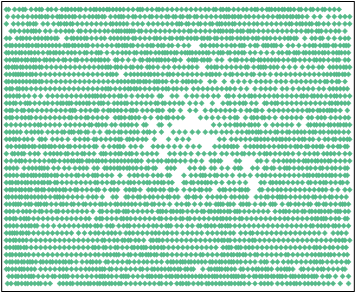
\includegraphics[width=0.5\columnwidth]{fig_multi_gate_placement_c7552}
\caption{Gate placement created by a commercial place-and-route tool for benchmark circuit c7552~\cite{brglez85}.}
\label{fig:multi_gate_placement_c7552}
\end{figure}
%\vskip 0.5em%

The list of gate placement coordinates is transformed into a sorted list of the nearest neighbors for each gate.
%
To perform a locality-based defect injection experiment, a random gate and defect polarity (STF or STR) are selected along with the nearest neighbors of the selected gate.
%
For each selected defect, the corresponding pre-computed TRAX delay (either a rising delay or falling delay) is added to the corresponding rising/falling delay of the selected gate using a testbench-level gate parameter override.
%
As already mentioned, the selected defects may belong to multiple recovery-level modules.

The simplistic approach used here differs from more advanced approaches such as~\cite{cai16}, where process variation is modeled in a hierarchical fashion, based on the work in~\cite{xiong07}.
%
In these approaches, the variation of an individual transistor is modeled as the sum of a hierarchy of random variables at the die level, the core level, and core-component level.
%
Modeling process variation at each level significantly reduces the complexity of analyzing spatially-correlated dependent random variables.
%
Such models require real-world measurements of IC variation, which can be accomplished using arrays of ring oscillators~\cite{bushan06} or by recording and analyzing near-infrared light emissions~\cite{stellari09}.
%
The approach presented here could be enhanced to receive input from such models and measurements to provide a more realistic selection of delay defects.
%
Further investigation of this topic is a rich area for future work.

\subsection{Defect distribution: Usage-based}
Defects induced or exacerbated by normal circuit operation, typically termed aging or wear-out defects, are targeted by usage-based defect injection.
%
For example, NBTI (negative bias temperature instability) affects the PMOS transistors of a logic gate, causing circuit speed degradation~\cite{borkar06, schroder03}.
%
While already an issue at 90nm~\cite{agarwal07}, the effects of NBTI continue to worsen as process technology continues to scales down~\cite{reddy02}.
%
The effects of NBTI increase while the PMOS transistor is turned on (has a logic-low input), and can be partially reversed while the transistor is turned off.
%
In an actual circuit, many of the PMOS transistors will become affected by NBTI during the life of the circuit.
%
However, not all affected transistors will result in an observable failure, as many of the slowdowns will affect non-critical paths and not affect any circuit output.

The ideal method of selecting defects to emulate usage-based degradation would start by tracking the usage of each PMOS transistor as the circuit is exercised with some workload.
%
Ideally, a realistic workload would be used to obtain the most accurate aging for each PMOS transistor.
%
This information would provide an estimate of the actual delay of each PMOS transistor affected by NBTI.
%
The resulting slowdowns can then be injected into the simulated circuit to determine if any failures occur.

The approach taken here differs slightly from the ideal approach.
%
To estimate usage-based transistor degradation, the TRAX fault simulator (Section~\ref{sec:trax_gpu}) is instrumented to track the number of ``ON'' cycles for the PMOS transistors in each gate.
%
Instead of a realistic workload, a test set of 100,000 random test pairs is generated and applied to each circuit using the instrumented fault simulator.
%
This results in a list of PMOS transistors potentially affected by NBTI, filtered to contain only those that spent more than 70\% of the test cycles in the ON state.
%
While this may not exactly match the transistor aging profile generated from a more realistic workload, we believe that the large number of random test vectors used provides a good characterization of the relative transistor aging in the circuit.
%
A histogram of the (unfiltered) PMOS transistor ON times for the circuit L2B~\cite{sun11} is shown in Figure~\ref{fig:multi_pmos_usage_l2b}.
%
It should be noted that any circuit workload (besides random) and threshold could be used instead of the ones chosen here.

%\vskip 0.5em%
\begin{figure}[hbtp]
\centering
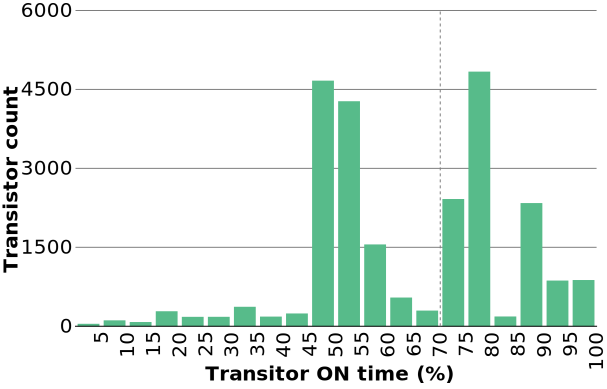
\includegraphics[width=0.8\columnwidth]{fig_multi_pmos_usage_l2b}
\caption{A histogram of the (unfiltered) PMOS transistor ON times for circuit L2B~\cite{sun11}.
%
The dashed line indicates the cutoff above-which transistors are considered NBTI-affected.}
\label{fig:multi_pmos_usage_l2b}
\end{figure}
%\vskip 0.5em%

To perform a usage-based defect injection experiment, $k$ random PMOS transistors are selected (without replacement) from the filtered set of NBTI-affected transistors\footnote{Random selection here is restricted to the set of NBTI-affected transistors, and is not a random selection of all circuit transistors.}.
%
This is slightly different from the previous two defect injection schemes.
%
Whereas random- and locality-based defect injection experiments add additional delay (either rising or falling) to a gate output, the usage-based defect injection experiments add delay only to a specific input-to-output transition for the affected gate.
%
That is, we perform transistor-level delay injection as opposed to gate-level delay injection.
%
This is accomplished through the following process.
%
For each of the $k$ random NBTI-affected transistors selected for an experiment, a custom logic gate is created, containing pin-to-pin timing specifications for the affected input transistor, based on the STR TRAX delay for that gate.
%
The STR TRAX delay is used because NBTI-affected PMOS transistors increase the gate output rise time\footnote{Care must be taken to consider how layout cell implementation may affect this assertion.
%
For example, if an AND gate is implemented by a NAND cell followed by an INV cell, the presence of extra PMOS transistors must be accounted for.}.
%
The original circuit design file is then programmatically modified to swap-in the customized gates, and gate-level simulation proceeds as normal.
%
As already described, the selected defects may belong to multiple recovery-level modules.
%
Note that in the ideal case, the aging of each PMOS transistor would determine the additional delay injected into the gate, while our experiments here use the TRAX delay (the minimum detectable delay for a fault site, empirically determined as part of the single defect injection experiments of Section~\ref{sec:diag_exp_diag}).


\section{Multiple Defect Diagnosis}
\label{sec:multi_diagnosis}
To reiterate, the end goal of on-chip diagnosis is to identify the failing modules of a core/uncore that has failed testing.
%
The result of performing each multiple-defect injection experiment described in Section~\ref{sec:multi_defect_injection_sites} is a pass/fail circuit response, consisting of one bit (pass or fail) for each applied test pair.
%
As detailed in Chapter~\ref{chap:diag}, diagnosis proceeds by analyzing the pass/fail result for each test pair in turn.
%
For each failing test, any candidate faults that are inconsistent with the test failure (that is, a Tester-Fail/Simulation-Pass situation) are eliminated from further consideration, that is, they are no-longer candidate faults.
%
Once all test responses are analyzed, the remaining candidate faults are used to generate a per-module count of candidate faults.
%
This part of the on-chip diagnosis process does not change in a multiple-defect context and remains the same as when diagnosing single defects in Section~\ref{sec:diag_exp_diag}.

As before, the per-module counts of candidate faults are used to evaluate the quality of the diagnosis result.
%
For the diagnosis experiments of Chapter~\ref{chap:diag}, where a single defect is injected for each experiment, a diagnosis result is deemed ``accurate'' if the defective module has a non-zero candidate fault count.
%
A diagnosis result is deemed ``ideal accurate'' if the defective module has the highest candidate fault count of all modules.

This evaluation process must be slightly altered when diagnosing multiple defects, because there is likely more than one defective module (i.e., a module that has one or more injected defects).
%
Here, ``accuracy'' is defined as a diagnosis result where all defective modules have non-zero candidate fault counts.
%
``Ideal accuracy'' is defined as a diagnosis result where all defective modules have candidate fault counts larger than the largest count of a non-defective module.
%
In other words, ideal accuracy occurs when no non-defective module would be placed higher than a defective module when ranked by candidate fault count.
% TODO add an image to show how this works, especially the "larger than the largest count of a non-defective module" part?

Additionally, a new ``partial accuracy'' metric is calculated for the multiple defect injection diagnosis results.
%
Whereas a single defect injection diagnosis is either inaccurate or accurate (the defective module has a zero or non-zero candidate fault count, respectively), the diagnosis result of an $n$-defect injection experiment may have from 0 through $n$ defective modules with a non-zero candidate fault count.
%
The partial accuracy metric is defined as the percentage of defective modules with non-zero candidate fault count.
%
For example, if a multiple defect injection experiment has five defective modules, a diagnosis result with all five modules having a non-zero candidate fault count would be classified as accurate with a partial accuracy of 100\%.
%
The partial accuracy metric is evaluated in addition to the existing metrics of accurate and ideal accurate, so it is possible that a 100\% partial accurate diagnosis (which would be deemed accurate) may also be ideal accurate, depending on the candidate fault counts of the non-defective modules.
%
Continuing the example, a diagnosis result with all five modules having zero candidate faults would be classified as inaccurate with a partial accuracy of 0\%.
%
Finally, a diagnosis result with, say, three of the five defective modules having a non-zero candidate fault count would be classified as inaccurate, but with a partial accuracy of 60\%.

It is entirely possible that one or more of the injected defects belong to the same module.
%
In these situations, for the purposes of computing the ``partial accuracy'' metric, the corresponding module of each injected defect is treated as an independent defective module.
%
For the example above with five injected defects, consider the situation where three of the five defects belong to module $A$, and two defects belong to module $B$.
%
With regard to ``partial accuracy,'' there are four possible scenarios.
%
First, if modules $A$ and $B$ both have zero candidate fault counts, the diagnosis result has a partial accuracy of 0\%.
%
Similarly, if both modules have non-zero candidate fault counts, the diagnosis result would have a partial accuracy of 100\%.
%
If only module $A$ has a non-zero candidate fault count, then three of the five defective modules are accurate, resulting in a partial accuracy of 60\%.
%
If only module $B$ has a non-zero candidate fault count, then two of five defective modules are accurate, leading to a partial accuracy of 40\%.
% TODO add an image to show this?

\section{Experiments}
\label{sec:multi_experiments}

Experiments are performed to evaluate the suitability of the TRAX fault model and the hierarchical dictionary for the task of diagnosing multiple injected defects.
%
Each experiment injects delay defects into a circuit and then performs gate-level simulation to determine if any incorrect responses are observed.
%
The result of this simulation is a list of pass/fail values, one for each simulated test-pair.
%
The fault dictionary is used with the pass/fail test responses to determine the set of TRAX faults that are compatible with the observed test results, that is, the presence of any of these compatible faults could explain the observed behavior.
%
Given that the end goal of TRAX on-chip diagnosis is to determine which module (or modules) are defective, the compatible faults are divided into groups based on the module where each belongs.
%
The counts of compatible faults belonging to each module are used to evaluate the quality of the diagnosis results, as explained in Section~\ref{sec:multi_diagnosis}.

The experiments presented here use c432 and c7552 from the ISCAS85 benchmark circuits~\cite{brglez85}.
%
Additionally, the L2B uncore from the OpenSPARC T2 processor design~\cite{sun11} is also used.
%
Twelve groups of defect injection experiments are performed for each of these three circuits, with 1,000 defect injections for each group.
%
The twelve groups for each circuit are divided into three groups of four (each group of four injecting 2, 5, 10, and 20 defects) for random-, locality-, and usage-based defect injections (as described in Section~\ref{sec:multi_defect_injection_sites}).

The diagnosis results for circuits c432, c7552, and L2B are shown in Figures~\ref{fig:multi_heatmap_c432}, \ref{fig:multi_heatmap_c7552}, and \ref{fig:multi_heatmap_l2b}, respectively.
%
Each figure has one column per experiment, grouped into random-, locality-, and usage-based defect injections, with 2-, 5-, 10-, and 20-injection experiments for each group.
%
The first two rows are the percent accurate (\%A) and percent ideal accurate (\%IA), followed by the partial accuracy histogram (as described in Section~\ref{sec:multi_diagnosis}).
%
Additionally, the partial accuracy histogram is shaded to highlight the larger bins, with darker background color indicating a higher percentage of diagnosis results.
%
The presence of empty (``$0.0$'') bins for the 2-, 5-, and 10-injection experiments is due to the quantization of partial accuracy, based on the number of injected defects.
%
For example, when injecting five defects the partial accuracy can have 0, 1, 2, 3, 4, or 5 modules correctly identified, corresponding to 0\%, 20\%, 40\%, 60\%, 80\%, or 100\% partial accuracy, respectively.

%\vskip 0.5em%
\begin{figure}[hbtp]
\centering
\includegraphics[width=\linewidth]{fig_multi_heatmap_c432}
\caption{Diagnosis results of multiple defect injection experiments for circuit c432.
%
Data rows labeled \%A and \%IA are the percentage of diagnosis results deemed accurate and ideal accurate, respectively.
%
The bottom row contains a small plot showing the distribution of the number of defective modules for each of the 1,000 experiments collated in the column.
%
The remaining rows are a normalized histogram of partial accuracy, shaded to highlight the larger bins.}
\label{fig:multi_heatmap_c432}
\end{figure}
%\vskip 0.5em%

%\vskip 0.5em%
\begin{figure}[hbtp]
\centering
\includegraphics[width=\linewidth]{fig_multi_heatmap_c7552}
\caption{Diagnosis results of multiple defect injection experiments for circuit c7552.
%
Data rows labeled \%A and \%IA are the percentage of diagnosis results deemed accurate and ideal accurate, respectively.
%
The remaining rows are a normalized histogram of partial accuracy, shaded to highlight the larger bins.}
\label{fig:multi_heatmap_c7552}
\end{figure}
%\vskip 0.5em%

%\vskip 0.5em%
\begin{figure}[hbtp]
\centering
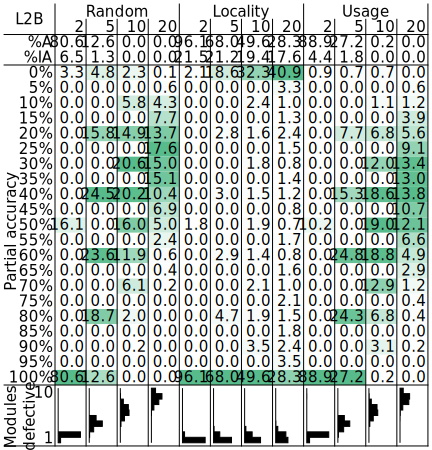
\includegraphics[width=\linewidth]{fig_multi_heatmap_l2b}
\caption{Diagnosis results of multiple defect injection experiments for circuit L2B.
%
Data rows labeled \%A and \%IA are the percentage of diagnosis results deemed accurate and ideal accurate, respectively.
%
The remaining rows are a normalized histogram of partial accuracy, shaded to highlight the larger bins.}
\label{fig:multi_heatmap_l2b}
\end{figure}
%\vskip 0.5em%

Below the partial accuracy histogram is a small plot showing the distribution of the number of defective modules for each of the 1,000 experiments collated in the column.
%
Due to the random selection of defects for injection, it is not guaranteed that all selected defects will be in separate modules.
%
Additionally, for the locality- and usage-based defect selection, it is expected that many of the selected defects will lie within the same module.
%
The maximum number of defective modules is the smaller of the number of modules in the circuit and the number of injected defects.
%
For example, each column of 2-injected defects has either one or two defective modules.
%
The defective module count plots reveal that for random defect selection, the number of defective modules also increases with the number of defects.
%
For the locality-based defect selection, there are fewer defective modules, meaning that the injected defects belong to the same few modules instead of being distributed throughout all modules.
%
The usage-based defect selection experiments show a defective module count distribution similar to the random experiments, but with a slightly smaller number of defective modules.

In general, the diagnosis results show better results for fewer defect injections (columns corresponding to 2- and 5-defect injections).
%
As more defects are injected, the partial accuracy histogram shows a shift from higher to lower partial accuracy.
%
Altogether, it appears that this approach is ineffective at diagnosing more than two delay defects.
%
However, it is important to note that the CASP on-chip test process~\cite{li08} uses periodic self-test with accelerated test conditions, in an effort to detect these gradual slowdowns before they affect correct system operation.
%
The periodic self-test will detect each defect as soon as it degrades sufficiently to produce incorrect output during the accelerated test, so ideally there will be only a few concurrent defects, maximizing the diagnostic ability of the TRAX fault model and hierarchical dictionary.

Comparisons are also drawn between the diagnosis results for random-, locality-, and usage-based defect selection.
%
For all three circuits analyzed, the diagnosis results for the locality-based defect injection experiments are more promising than the random- or usage-based experiments.
%
This is because gates in the same hierarchical module are likely to be placed in close proximity by the place-and-route tool to minimize wiring distances, logically leading to more injected defects belonging to the same module.
%
When many injected defects lie within the same module, it is likely that more candidate faults will belong to that defective module, increasing the diagnosis quality.

The diagnosis results for the usage-based defect injection experiments for c432 bear further analysis.
%
As shown in the rightmost four columns of Figure~\ref{fig:multi_heatmap_c432}, the diagnosis results are entirely bimodal, with each diagnosis result being either 0\% partially accurate or 100\% partially accurate.
%
When analyzing the most-aged PMOS transistors (based on transistor ON time during test application, details in Section~\ref{sec:multi_defect_injection_sites}), it happened to be that the top 30\% most-aged transistors are all located within the same module.
%
This is possibly due to the relatively smaller size of this circuit (208 gates), as this behavior is not observed for either of the other two circuits.


\subsection{Interaction of Multiple TRAX Faults}
The experiments presented here are an evaluation of the ability of the un-modified TRAX fault model and hierarchical fault dictionary to diagnose the response of multiple injected defects.
%
Another potential approach to this problem might involve modifying the diagnosis process and on-chip diagnosis architecture to better encompass the fault effects of multiple defects.
%
Here, we analyze the efficacy of the TRAX-based dictionary for the diagnosis of multiple delay defects, each of which is modeled by a TRAX fault.
%
Specifically, the interaction of fault effects (i.e., unknown values \textit{X}) from more than one activated TRAX fault is analyzed.

Due to the conservative propagation of the faulty \textit{X} value, a TRAX fault response subsumes any possible response of a co-located delay defect.
%
That is, the observed response of any defect must be a subset of the corresponding TRAX fault response, and it is not expected to be an exact match.
%
This is the basis of the TFSP diagnosis process outlined before, where an observed test failure will eliminate any modeled faults that could not have produced a failure for that test.

The combined response of two or more TRAX faults is simply the union of the failing values (due to the non-destructive and non-masking interactions of \textit{X} values).
%
However, unlike the single defect situation, where the defect response must be a subset of the corresponding TRAX fault response, the situation is more complex when analyzing the response of multiple defects.
%
No assumptions are made about which TRAX faulty outputs will fail due to the presence of the corresponding defects.
%
Because of this, it is possible that the defective circuit will fail any combination of the potentially failing tests from the union of TRAX fault responses.
%
This may result in a defective circuit test response, that when used with the TFSP-based on-chip diagnosis, eliminates all candidate faults due to the test response being incompatible with all modeled faults.

%\vskip 0.5em%
\begin{table}[hbtp]
\centering
\begin{tabular*}{0.9\columnwidth}{@{\extracolsep{\fill}}cccccccl}
\toprule
Fault&Module&$T_1$&$T_2$&$T_3$&$T_4$&$T_5$&\\
\midrule
$F_1$&$M_1$&P&F&F&P&F&\\
$F_2$&$M_1$&P&F&F&P&F&Eliminated (EQU)\\
$F_3$&$M_1$&P&F&P&P&P&Eliminated (SUB)\\
$F_4$&$M_1$&F&F&P&P&F&\\
\midrule
$F_5$&$M_2$&F&F&P&P&F&\\
$F_6$&$M_2$&P&P&F&F&P&\\
\bottomrule
\end{tabular*}
\caption{TRAX fault dictionary data illustrates dictionary compaction, using equivalence and subsumption relationships to eliminate two intra-module faults.}
\label{table:multi_fault_resp}
\end{table}
%\vskip 0.2em%

As an example, consider two faults from Table~\ref{table:multi_fault_resp}, $F_1$ and $F_4$.
%
These faults belong to the same module, and because they are not equivalent and neither subsumes the other, the dictionary compaction process does not eliminate either.
%
Their pass/fail responses (represented by `P' and `F', respectively, in the table rows) show at least one test where one fault could produce a failure and the other fault could not (i.e., $F_1$ uniquely fails $T_3$, and $F_4$ uniquely fails $T_1$).
%
For example, if a circuit is affected by defects at the same locations as $F_1$ and $F_4$, testing might produce a test response of ``PFPPF'', ``FPPPF'', or ``FFFPP'', among other possible test responses.
%
Diagnosing the third possible test response ``FFFPP'', the first failure would eliminate $F_1$ as a candidate fault, and the third failure would eliminate $F_4$, due to a Tester-Fail/Simulation-Pass (TFSP) condition for both faults.

Again, given the conservative propagation properties of the unknown value \textit{X}, the set of failing outputs is only a ``worst case'' accounting of the fault response.
%
The actual set of failing circuit outputs and failing tests will likely be much smaller, enabling accurate diagnosis of multiple failures, as demonstrated in Section~\ref{sec:multi_experiments}.
%
The use of such an approach, where multiple TRAX faults are merged and stored in the dictionary, deserves further investigation.
%
However, the approach may suffer from a much larger dictionary due to the $n \times (n - 1)$ fault pairs modeled.
%
Alternatively, modifications might be made to the diagnosis architecture to perform the TRAX fault effect merging during diagnosis.


\section{Summary}
\label{sec:multi_summary}

While the experiments of Section~\ref{sec:diag_exp_diag} performed single-defect injection diagnosis, a natural extension of that work is to consider how well on-chip diagnosis performs with a circuit that is affected by multiple defects.
%
The hypothesis here is to see if the TRAX fault model, the hierarchical dictionary, and the on-chip diagnosis process is similarly effective at localizing defects to the recovery-level module(s).
%
To provide for more realistic multiple-defect injection experiments, three defect selection approaches are developed, including a simple random selection, plus a locality-based defect selection process targeting gate oxide defects, and a usage-based defect selection process targeting NBTI slowdown defects.
%
These three approaches (random, locality, usage) are used to perform over 30,000 multiple defect injection experiments.

The results of the defect injection experiments are diagnosed by the on-chip diagnosis process, using a standard TRAX hierarchical fault dictionary.
%
While the first half of the on-chip diagnosis process (using occurrences of Tester-Pass/Simulation-Fail (TPSF) to eliminate faults from further consideration) remains the same, the diagnosis evaluation metrics of ``accuracy'' and ``ideal accuracy'' are updated to work in the context of multiple defective modules.
%
For example, a diagnosis result where all defective modules have non-zero candidate fault counts would be deemed accurate.
%
Additionally, a partial-accuracy metric is also developed to provide a measure of accuracies between 0\% and 100\% accurate.
%
Diagnosis results typically achieve more than 90\% accuracy when diagnosing two injected defects, with especially promising results for locality-based defect injection.
%
Altogether, the TRAX fault model, the hierarchical dictionary, and on-chip diagnosis are shown to be an effective tool for diagnosing two concurrent defects.
%
It is possible, however, to improve on these results by developing an approach that directly analyzes the effects of multiple defects.


\chapter{Conclusions}
\label{chap:conclusions}

Ensuring robustness of integrated circuits as fabrication technology continues to scale has been, and will continue to be, an important aspect in the advancement of computing systems.
%
The approach to ensuring robustness used here centers around periodic on-chip self-test and diagnosis.
%
First, a fault must be detected by high-quality test vectors loaded in from off-chip, applied to the core/uncore under test using the existing design-for-test (DFT) hardware.
%
Second, the test responses must be analyzed to localize the failure within the core/uncore.
%
Third, the affected portion of the system must be repaired, replaced, or avoided to ensure the system remains functional even when affected by one or more faults.
%
Finally, to ensure correctness in the ongoing computation, a recovery step may be necessary to recover the system state.
%
This is the approach presented in CASP (Concurrent Autonomous Chip Self-Test Using Stored Test Patterns)~\cite{li08, inoue08, li10casp, li13}.
%
CASP is assumed as a starting point for the work presented in this dissertation which is focused on diagnosis performed inside the chip.

To perform failure diagnosis in an on-chip context requires an approach with minimal processing and storage requirements.
%
Fault diagnosis approaches are categorized as either effect-cause or cause-effect approaches.
%
In an effect-cause approach, diagnosis software will analyze the complete model of the circuit design, along with the complete test set and faulty circuit output, to reason about the structure of the circuit and how the observed faulty behavior could propagate through the circuit.
%
This requires signficant computational resources and is not suitable for on-chip diagnosis.
%
The other diagnosis approach is cause-effect, where fault simulation is used to hypothesize how a circuit would behave if affected by one of many modeled faults.
%
This builds a catalog of faulty circuit responses, called a fault dictionary.
%
This tabular data is easily compared against the observed faulty behavior, and modeled faults that match (or are close to matching) the actual failing-circuit response are identified as likely locations of the detected failure.
%
Unlike the complex software analysis required for effect-cause diagnosis, the use of a fault dictionary is very simple, requiring only very limited hardware or software support.

The approach taken here in this dissertation is to construct and store a fault dictionary for use in on-chip diagnosis.
%
For the targeted early-life and wear-out failures, which manifest as gradually increasing delay through circuit gates, a flexible and generalized fault model such as TRAX is effective in capturing the uncertainty of delay.
%
In the specialized context of on-chip diagnosis, the limited storage space and relaxed diagnosis requirements mean that a compacted fault dictionary need only localize failures to the level of recovery, that is, to the level of repair, replacement, or avoidance.
%
This diagnostic relaxtion permits the dictionary to eliminate many faults that do not contribute to distinguishing intra-module faults, reducing the dictionary size.
%
The use of a hierarchical dictionary for on-chip diagnosis is performed by a scalable diagnosis architecure, designed to be a low-overhead addition to the CASP test system~\cite{li08}.
%
At the cost of less than 0.05\% chip area overhead for the OpenSPARC T2 processor design, the diagnosis architecture localizes any failures to the repair-level, enabling the repair, replacement, or avoidance of the core/uncore to ensure that the system remains robust.
%
The rest of this concluding chapter describes the dissertation contributions and directions for areas of future work.


\section{Dissertation Contributions}
\label{sec:conclusions_dissertation_contrib}

The combination of the TRAX fault model, hierarchical fault dictionary, and on-chip diagnosis architecture results in a comprehensive methodology to efficiently diagnose failures to the required level of the design hierarchy.
%
A fast fault simulator greatly reduces the computation time needed to generate a TRAX fault dictionary, and the on-chip diagnosis process has been evaluated for suitability in diagnosing multiple concurrent failures.
%
The major contributions of this dissertation include:

\textbf{TRAX Fault Model}
\begin{itemize}
\item{\textit{Activation and propagation rules:} Targeting the gradual gate slowdowns caused by early-life and wear-out failures, the TRAX fault model is designed to encompass all potential fault effects of a delay defect.
%
The TRAX fault model is similar to the unspecified-transition fault model~\cite{pomeranz08} but includes hazard activation in addition to conventional transition activation to ensure full subsumption of delay defects.
%
The \textit{X} value generated at fault activation conservatively prevents error masking that might occur with the TF model, resulting in a very conservative propagation of fault effects to circuit outputs.
%
The TRAX subsumption of TF faults is experimentally validated for a variety of circuits.}
\item{\textit{GPU-accelerated fault simulation:} The incredible parallelism of graphics processing units (GPUs) is harnessed to provide an efficient fault simulation engine to accelerate the computationally demanding process of creating a fault dictionary.
%
Runtime comparisons with a leading commercial tool show an average speedup of nearly 8x (maximum of 19x) for the GPU accelerated TRAX fault simulator.}
\item{\textit{Comparison of TRAX and TF fault effect subsumption:} To further explore and validate the TRAX subsumption of TF fault responses, we perform a series of circuit simulation experiments using several benchmark circuits.
%
For every selected fault site, TRAX and TF fault simulations are performed, and the simulated circuit outputs are compared between TRAX and TF.
%
For each fault analyzed in this way, the TRAX response subsumed the TF response in terms of the number of fault detections, confirming the ability of TRAX to fully-subsume the fault effect behavior of the transition fault model.}
\end{itemize}

\textbf{Hierarchical Fault Dictionary}
\begin{itemize}
\item{\textit{Exploitation of module-level hierarchy for relaxation of required diagnostic precision:} The recovery actions available to a faulty system-on-chip (SoC) at runtime, including repair, replacement, or avoidance of a defective module, are all quite granular in scope.
%
For example, it is not economically feasible to repair a single slowed transistor or swap out a spare gate for an un-damaged one.
%
Therefore, it is not necessary to distinguish between modeled faults belonging to the same repair-level module.
%
This permits additional dictionary compaction techniques, as well as enables the use of the on-chip diagnosis architecture to perform repair-level diagnosis.}
\item{\textit{Hierarchical dictionary compaction through fault elimination via equivalence and subsumption:} Significant dictionary size reduction can be achieved by analyzing intra-module fault pairs and eliminating faults due to equivalence and subsumption.
%
Within a module, all-but-one test-set equivalent fault (those having identical simulation responses for all tests) can be eliminated.
%
Additionally, a fault with an erroneous test response wholly subsumed by another intra-module fault can be eliminated from the set of modeled faults.
%
Equivalence/subsumption fault elimination further compacts the fault dictionaries by an additional 92\% on average.}
\item{\textit{Dictionary size reduction by up to four orders of magnitude:} Leveraging pass/fail compaction with equivalence and subsumption fault elimination can drastically reduce the storage size required for a fault dictionary.
%
This is especially valuable for on-chip diagnosis when all dictionary data must be stored off-chip in DRAM, flash, or on disk.
%
On average, the dictionary size is reduced by 99.37\% for UTF and reduced by 99.85\% for TRAX.
%
The maximum reduction for a UTF dictionary is the NCU dictionary, which is compacted down to only 0.003683\% of the original size, a reduction by over 27,000x.
%
This reduces the NCU fault dictionary from 211 GB for the full-response dictionary to under 8 MB for the UTF compacted pass/fail dictionary.}
\end{itemize}

\textbf{On-Chip Diagnosis Architecture}
\begin{itemize}
\item{\textit{TRAX on-chip diagnosis architecture:} A scalable, low-overhead diagnosis architecture has been designed to diagnose the pass/fail test responses of any faulty core/uncore.
%
Using hierarchical dictionary data loaded in from off-chip, the fault accumulator hardware iteratively searches for instances of Tester-Fail/Simulation-Pass (TFSP).
%
Each TFSP occurrence indicates a modeled fault that is not compatible with the observed test failures.
%
Once the set of candidate faults is determined, the Faulty Module Identification Circuit (FMIC) analyzes the candidate fault set to determine the per-module candidate fault counts, which are used to make decisions about how to recover the core/uncore.}
\item{\textit{Tradeoffs in chip area and diagnosis time overhead:} The fault accumulator component of the on-chip diagnosis architecture is scalable in terms of the number of candidate faults under concurrent evaluation.
%
By scaling the number of concurrent faults handled in the fault accumulator, a tradeoff can be made between chip area overhead and cycles required for diagnosis.
%
For one of the largest circuits analyzed (the OpenSPARC T2 uncore ``NCU'', with 211 tests, 21,537 faults, and ten modules), diagnosis hardware requires approximately 26,000 cycles to perform diagnosis, and approximately 38,000 gates, an overhead of less than 0.0077\% for the OpenSPARC T2 design.}
\item{\textit{Diagnosis of injected delay defects:} More than 32,000 delay-defect injection experiments are performed, across three circuits, to create realistic failing test responses to evaluate the on-chip diagnosis process.
%
Diagnosis results for these experiments are 100\% accurate, showing that the TRAX fault model subsumes all potential effects of a delay defect.
%
Further analysis shows promising results for UTFs, including improved diagnosis resolution at the expense of sub-perfect accuracy.
%
Normalization of per-module candidate defect counts also shows general improvement to diagnosis results for TRAX faults.}
\end{itemize}

\textbf{Multiple Defect Diagnosis}
\begin{itemize}
\item{\textit{Realistic defect-site selection for defect injection:} To provide the most realistic defect-injection experiments, the distribution of injected defects should reflect the distribution of the targeted defect types (namely, early-life and wear-out failures).
%
Three schemes are investigated and implemented, random-, locality-, and usage-based defect site selection.
%
Random defect selection provides a baseline for comparison, while locality-based defect selection uses a commercial place-and-route tool to preferentially select clusters of nearby defect sites, in an effort to emulate early-life and other defects caused by fabrication process variation.
%
Usage-based defect selection analyzes the transistor on-time characteristics to identify PMOS transistors most likely to be affected by wear-out (aging) defects such as Negative Bias Temperature Instability (NBTI).}
\item{\textit{On-chip diagnosis of multiple injected defects:} Over 30,000 multiple-defect injection experiments are performed, using on-chip diagnosis to determine the most likely defective module(s).
%
Despite being designed to capture the misbehaviors of only a single delay defect, the TRAX fault model is effective in diagnosing multiple injected defects, typically achieving more than 90\% accuracy with reasonable resolution for two injected defects, with especially promising results for locality-based defect injection experiments.}
\end{itemize}


\section{Final Remarks}
\label{sec:conclusions_concluding_remarks}

Two major trends in the computing world include the continung scaling-down of chip features causing reduced reliability, and the increasing computerization of various domains including safety-critical systems such as autonomous vehicles and implantable medical devices.
%
Taken together, these trends contribute to an intense need for ensuring robust operation of such critical systems.
%
As we continue to put computers inside our bodies (medical devices), and put our bodies inside large mobile computers (modern vehicles, airliners, etc), ensuring robustness becomes one of the most-important system characteristics.

Periodic on-chip test and diagnosis is a promising approach to ensure such robustness, by detecting failures as they occur (or are about to occur), localizing the failure to specific modules of the chip, and performing some sort of recovery operation.
%
The localization step is performed using on-chip diagnosis, requiring relatively little in the way of off-chip storage or diagnosis hardware.
%
The cause-effect dictionary diagnosis uses an efficient and scaleable fault diagnosis architecture to determine the faulty components of the design.

As chips continue to become smaller and faster they end up being less naturally reliable.
%
With increased deployment of unreliable computing systems within safety-critical domains, it is hoped that the on-chip diagnosis technique at the core of this thesis can be extended and enhanced to provide robust operation.


\section{Future Work}
\label{sec:conclusions_future_work}

This dissertation provides a comprehensive study of the use of on-chip diagnosis using a TRAX-based hierarchical fault dictionary for localizing early-life and wear-out failures.
%
Here, some possible future extensions and related topics are described.

\begin{itemize}
\item{\textit{Investigate tradeoffs in TRAX fault model variants:} While this dissertation investigated the difference between TRAX and UTF fault models, in terms of dictionary size and diagnostic abilities, there are other variants that might be interesting to investigate.
%
For example, the GPU-accelerated TRAX fault simulator generates a hazard \textit{H} value at a gate output if it detects a non-constant controlling value on at least one gate input.
%
This is implemented by detecting each possible hazard-generating input combination, for example for a two-input gate, the transitions 01 $\rightarrow$ 10 and 10 $\rightarrow$ 01 clearly have no constant controlling value inputs.
%
Further, what should the behavior be for input transitions like 0H $\rightarrow$ 10 or H0 $\rightarrow$ 0H?}
\item{\textit{Investigate faults that fail most applied tests:} Some dictionary compaction experiments result in an astonishingly small dictionary, determined to be due to the presence of TRAX ``super faults'' that resulted in failing circuit outputs for most applied tests.
%
Further investigation showed that this is due to a combination of factors, most notably the presence of many hazard values in the affected circuits, coupled with circuits composed of predominantly XOR gates.
%
As shown in Figure~\ref{fig:trax_gate_evaluation} on page~\pageref{fig:trax_gate_evaluation}, any \textit{H} inputs to an XOR or XNOR gate will result in propagating that \textit{H} to the gate output (unless there is an \textit{X} input), which results in the activation of the gate output fault.
%
It could be investigated to determine if these ``super faults'' are present in many circuits or just the few affected circuits observed, and to determine if the hazard-generation conditions are too pessimistic, leading to such super faults.}
\item{\textit{Further improve GPU-accelerated fault simulator:} While achieving nearly 8x speed-up on average, the GPU fault simulator is not as fast as it could be.
%
There are a variety of areas of improvement in the GPU programming that could be implemented with further investigation and research.
%
For example, some existing non-GPU fault simulators take advantage of wide math instructions (performing the same operation on multiple operands) to improve simulation speed, such as by using bitwise operators to perform 32 or 64 gate evaluations per thread of execution.
%
Another idea is to improve the alignment and cohesion of memory accesses across threads, as there are strict guidelines to follow to ensure maximum memory bus utilization.
%
Further investigation is warranted for the special-purpose memory types such as constants and texture memories, which may be especially well-suited for constant data such as the circuit netlist or gate evaluation lookup table.}
\item{\textit{Usage-based defect injection workload:} The usage-based defect site selection used PMOS transistor ON-time data gathered by the GPU fault simulation, generated from random test vectors.
%
To increase the accuracy of the transistor-aging metric, it would be best to use a realistic workload instead of random tests.
%
Additionally, while the current set of aged PMOS transistors are selected based on static criteria (``turned on more than 70\% of test vectors''), a more realistic set of aged transistors could be obtained by also considering the position of each gate within the circuit, for example if it is part of a (near) critical path or on a path with plenty of timing slack.}
\item{\textit{TRAX-aware test pattern generation:} The current approach uses conventional Automatic Test Pattern Generation (ATPG) targeting transition faults.
%
This results in a test set with high coverage of individual transition faults.
%
However, this is not the end goal of on-chip diagnosis.
%
While the hierarchical fault dictionary compaction process eliminates many modeled faults in the context of module-level diagnosis, it would likely be more effective to make all parts of this process aware of the overall diagnosis requirements (failure localization only to the level of repair, replacement, or avoidance).
%
Perhaps the ATPG process could be modified to prioritize test vectors that distinguish inter-module faults.}
\item{\textit{Adaptive TRAX on-chip test and diagnosis:} The use of a static (but patchable) test set and fault dictionary requires that the selected core/uncore be tested with the entire test set, and run through the entire diagnosis process, even if the first $n$ tests unambiguously determine the defective module.
%
Modifying the CASP test architecture to incorporate the TRAX on-chip diagnosis architecture as part of a combined test+diagnosis process might enable adaptive test application, or provide for an early exit if the defective module becomes known before the end of the test set, potentially saving significant core/uncore downtime.}
\end{itemize}



%\newpage
%\pagestyle{plain}
%TODO add bibliography to ToC like Cheng?
\bibliographystyle{ieeetr}
\bibliography{dissertation}

\end{document}
